\documentclass[british]{ntnuthesis}

\title{Parallel Processing and Anomaly Detection of DAS Data using Autoencoders: Enhancing Efficiency in Large-Scale Sensor Data Analysis}
\shorttitle{Parallel Processing and Anomaly Detection on DAS data}
\author{Jørgen Aleksander Fagervik \\
        Supervisor: Ole Jakob Mengshoel \\
        Co-supervisor: Anne Cathrine Elster}
\shortauthor{J. A. Fagervik}
\date{CC-BY \ntnuthesisdate}

\addbibresource{thesis.bib}


% From https://www.overleaf.com/learn/latex/Glossaries

\makeglossaries % Prepare for adding glossary entries

\newglossaryentry{julia}
{
        name=Julia,
        description={Is an all-purpose programming language specially suited for
scientific computing}
}

\newglossaryentry{python}
{
        name=Python,
        description={Is an all-purpose general programming language suited for scripting, data-science and web applications}
}

\newglossaryentry{llvm}
{
        name=LLVM,
        description={Low Level Virtual Machine, better known as LLVM, is a project trying to provide a modern, SSA-based compilation strategy capable of supporting both static and dynamic compilation of arbitrary programming languages \cite{llvm}}
}

\newglossaryentry{fftw}
{
        name=FFTW,
        description={Fastest Fourier Transform in the West is one of the most famous implementations of the \acrshort{dft} algorithm. It is specialized for running on \acrlong{cpu}s}
}

\newglossaryentry{relu}
{
    name=ReLU,
    description={Rectified Linear Unit is one of the most commonly used activation functions within \acrshort{dnn}s}
}

\newglossaryentry{bibliography}
{
        name=bibliography,
        plural=bibliographies,
        description={A list of the books referred to in a scholarly work,
typically printed as an appendix}
}

\newglossaryentry{maths}
{
    name=mathematics,
    description={Mathematics is what mathematicians do}
}
\newglossaryentry{pubdas}
{
    name=PubDAS,
    description={A PUBlic Distributed Acoustic Sensing Datasets Repository for Geosciences}
}

\newglossaryentry{idun}{
    name=IDUN,
    description={The Idun cluster is a project between NTNU's faculties and the IT division that aims at providing a high-availability and professionally administrated compute platform for NTNU}
}

\newglossaryentry{svm}
{
    name=Support Vector Machine,
    description={Common machine learning technique}
}




% --------------------
% ----- Acronyms -----
% --------------------

\newacronym{ntnu}{NTNU}{Norwegian University of Science and Technology}
\newacronym{ai}{AI}{Artificial Intelligence}
\newacronym{ast}{AST}{Abstract Syntax Tree}
\newacronym{mb}{MB}{Megabyte}
\newacronym{gb}{GB}{Gigabyte}
\newacronym{tb}{TB}{Terrabyte}
\newacronym{ml}{ML}{machine learning}
\newacronym{fft}{FFT}{Fast Fourier Transform}
\newacronym{rfft}{RFFT}{Fast Fourier Transform for Real Numbers}
\newacronym{dft}{DFT}{Discrete Fourier Transform}
\newacronym{mpi}{MPI}{Message-passing interface}
\newacronym{ram}{RAM}{Random-access memory}
\newacronym{gcd}{GCD}{Greatest Common Divisor}
\newacronym{hpc}{HPC}{High Performance Computing}
\newacronym{api}{API}{Application program interface}
\newacronym{gpu}{GPU}{Graphics processing unit}
\newacronym{tpu}{TPU}{Tensor processing unit}
\newacronym{cpu}{CPU}{Central processing unit}
\newacronym{das}{DAS}{Distributed acoustic sensing}
\newacronym{ann}{ANN}{Artificial neural network}
\newacronym{cnn}{CNN}{Convolutional neural network}
\newacronym{rnn}{RNN}{Recurrent Neural Network}
\newacronym{dnn}{DNN}{Deep Neural Network}
\newacronym{repl}{REPL}{Read-eval-print loop}
\newacronym{lstm}{LSTM}{Long short-term memory}
\newacronym{jit}{JIT}{Just-in-time}
\newacronym{hdf}{HDF}{Hierarchical Data Format}
\newacronym{hdf5}{HDF5}{Hierarchical Data Format version 5}
\newacronym{sisd}{SISD}{Hierarchical Data Format version 5}
\newacronym{simd}{SIMD}{Single instruction, multiple device}
\newacronym{misd}{MISD}{Multiple instructions, single device}
\newacronym{mimd}{MIMD}{Multiple instructions, multiple device}
\newacronym{spmd}{SPMD}{Single program, multiple device}
\newacronym{cgf}{NTNU CGF}{NTNU Centre for Geophysical Forecasting}
\newacronym{posix}{POSIX}{Portable Operating System Interface}
\newacronym{asn}{ASN}{ALCATEL SUBMARINE NETWORKS}
\newacronym{dsp}{DSP}{Digital Signal Processing}
\newacronym{adam}{ADAM}{Adaptive Moment estimation}
\newacronym{sgd}{SGD}{Stochastic Gradient Descent}
\newacronym{gru}{GRU}{Gated Recurrent Unit}
\newacronym{llm}{LLM}{Large Language Model}
\newacronym{sota}{SOTA}{State of the Art}
\newacronym{dl}{DL}{Deep Learning}
\newacronym{vae}{VAE}{Variational Autoencoder}
\newacronym{mae}{MAE}{Mean Absolute Error}
\newacronym{mse}{MSE}{Mean Squared Error}
\newacronym{gan}{GAN}{Generative Adverserial Network}
\newacronym{dbscan}{DBSCAN}{Density-Based Spatial Clustering of Applications with Noise}
\newacronym{adagrad}{AdaGrad}{Adaptive Gradient Algorithm}
\newacronym{fir}{FIR}{Finite Impulse Response}
\newacronym{elbo}{ELBO}{Evidence Lower BOund}
\newacronym{roi}{ROI}{Range of Interest}
\newacronym{rf}{RF}{Radio Frequency}
\newacronym{kld}{KLD}{Kullback-Leibler Divergence}

\newacronym{pr}{PR}{Precision-Recall}
\newacronym{auc}{AUC}{Area-Under-Curve}
\newacronym{cae}{CAE}{convolutional autoencoder}
\newacronym{cvae}{CVAE}{convolutional variational autoencoder}
\newacronym{fcnn}{FCNN}{Fully Connected Neural Networks}
\newacronym{foss}{FOSS}{free and open-source software}

 % add glossary and acronym lists before document
\usepackage{listings}
\usepackage[table,xcdraw]{xcolor}
\usepackage{siunitx}
\usepackage{multirow}
\usepackage{pgfplots}
\usepackage{algorithm}
\usepackage{algpseudocode}
\usepackage{textcomp}
\usepackage{tikz}
\usepgfplotslibrary{groupplots}
\usepackage{booktabs}
\usepackage{colortbl}
\usepackage{array}
\usepackage{makecell}
\usepackage{xcolor}
\usepackage{caption}

% Define a custom color for the caption background
\definecolor{captionbg}{RGB}{240,240,240}
\definecolor{captiontext}{RGB}{0,0,0}
\definecolor{captionframe}{RGB}{100,100,100}

\newcommand{\mycomment}[1]{}
% Define a custom caption style
\DeclareCaptionFormat{thesiscaption}{%
    \begin{tikzpicture}
    \node[inner sep=10pt, fill=captionbg, draw=captionframe, line width=0.5pt, rounded corners] {%
        \parbox{\dimexpr\textwidth-20pt\relax}{%
            \textbf{\color{captiontext}#1#2}%
            \par\vskip2pt%
            \color{captiontext}#3%
        }%
    };
    \end{tikzpicture}%
}

% Apply the custom style to listings and figures
\captionsetup[lstlisting]{format=thesiscaption, labelfont={bf}, textfont={}, justification=justified, singlelinecheck=false}

% Define Julia style
\lstdefinelanguage{Julia}{
  keywords={abstract, break, case, catch, const, continue, do, else, elseif, end, export, false, for, function, global, if, import, in, macro, module, otherwise, quote, return, true, try, using, while, type, mutable, struct, @inline, @simd, @time, @btime, @layer, @functor, @error, @warn, @show, @inbounds, @kwdef, @view, @layout, @gif,
  Real, Integer, Int, Int8, Int16, Int32, Int64,
  String, AbstractString,
  DateTime, Second, Minute, Hour, Date,
  Bool, Tuple, Matrix, Dict, Set, Vector, AbstractArray, AbstractVector, AbstractMatrix,
  AbstractFloat, Float, Float8, Float16, Float32, Int64,
  },
  sensitive=true,
  comment=[l]\#,
  morecomment=[s]{\#=}{=\#},
  morestring=[b]",
}

\definecolor{backcolour}{rgb}{0.99,0.99,0.99}
\definecolor{codegreen}{rgb}{0,0.6,0}

% Define a custom style
\lstdefinestyle{dasstyle}{
    backgroundcolor=\color{backcolour},   
    commentstyle=\color{codegreen},
    basicstyle=\ttfamily\footnotesize,
    breakatwhitespace=false,         
    breaklines=true,                 
    keepspaces=true,                 
    numbers=left,
    frame=single,
    numbersep=5pt,                  
    showspaces=false,                
    showstringspaces=false,
    showtabs=false,                  
    tabsize=2,
}

% Define colors for the command prompt
\definecolor{promptcolor}{rgb}{0.5,0,0}
\definecolor{commandcolor}{rgb}{0,0,0.5}

% Configure the listing style for shell commands
\lstdefinestyle{shellcommand}{
  basicstyle=\ttfamily\small,
  breaklines=true,
  captionpos=t,
  commentstyle=\color{promptcolor},
  keywordstyle=\color{commandcolor},
  stringstyle=\color{commandcolor},
  numbers=none,
  numbersep=5pt,
  numberstyle=\tiny\color{black},
  frame=single,
  framesep=5pt,
  xleftmargin=15pt,
  framexleftmargin=15pt,
  backgroundcolor=\color{gray!10},
  showspaces=false,
  showstringspaces=false,
  showtabs=false,
  tabsize=2,
  breakatwhitespace=false,
  escapeinside={(*@}{@*)},
}

% Use \lstset to make myStyle the global default
\lstset{style=dasstyle}

\newcommand{\rnum}[1]{\uppercase\expandafter{\romannumeral #1\relax}}
\begin{document}


\begin{titlepage}
\newgeometry{left=1.6in, right=2in}
\vspace*{1.5cm}

\noindent  \textcolor{gray}{\large Jørgen Aleksander Fagervik} \\
\vspace{1cm}

\noindent \textbf{\Large Parallel Processing and Autoencoder-based Anomaly Detection for Distributed Acoustic Sensing Data} \\
\vspace{0.5cm}

\noindent {Designing Scalable Programs for Enhanced Efficiency in Large-Scale \acrshort{das} Data Processing and  Analysis} \\



\vspace{7cm}
\noindent Master's thesis in Computer Science \\
Supervisor: Ole Jakob Mengshoel \\
Co-supervisor: Anne Cathrine Elster \\
September 2024 \\

\vspace{0.2cm}
\noindent Norwegian University of Science and Technology \\
Faculty of Information techonolgy and electrical engineering \\
Department of Computer Science (IDI) \\

\begin{figure}[h]
\includegraphics[scale=0.5]{figures/ntnu.png}
\end{figure}
\end{titlepage}
\restoregeometry
\myemptypage 

\chapter*{Preface}

This master thesis was prepared during the spring of 2024 at the \acrfull{ntnu}, Faculty of Information Technology and Electrical Engineering, Department of Computer Science. The thesis was written and accomplished in cooperation with NTNU SFI Centre for Geophysical Forecasting. \\

This marks the end of a long journey. Through ups and downs I've made it to where I'm at today, writing these very words. I distinctly remember the day I entered university. I did not know what I'd like to focus on, given my various different interests within computing from the age of 14. I stand here now, trying to bridge the gap between HPC and AI, with this thesis as my weapon in this fight. \\

I want to give my sincerest thanks to my supervisor Ole Jakob Mengshoel for listening to my monologues and providing guidance thorughout this last year of my studies. Robin Rørstadbotnen for helping me get the necessary data and how to get started. Martin Landrø at \acrlong{cgf} for providing me with data and resources, and Helene for all clearance related stuff. Besides these people, I want to offer my gratitude towards my friends and family for always sticking by my side, no matter what life threw at me. Without them, I'd be lost on the path of life. \\

Last of all I want to thank my girlfriend, Ronja, the beacon of my heart for staying by my side through good and bad days throughout this semester and for always supporting me.\\

Finally, as I leave my final lasting remarks before I graduate, I can only think of a few wise words regarding the future.
\quote{\textit{To infinity and beyond!} - Buzz Lightyear}

\begin{flushright}
Trondheim, Fall 2024  \\
\textit{Jørgen Aleksander Fagervik}
\end{flushright}
\chapter*{Abstract}

Signal processing and \acrfull{ai} has become .

Parts of this thesis are taken from or based on my submitted project assignment in the subject TDT4501 with the title "Parallel DAS Processing: Julia is all you need".
\chapter*{Sammendrag}

Denne avhandlingen undersøker parallell prosessering av distribuert akustisk sensing (DAS)-data og anvendelsen av autoencodere for anomalideteksjon på disse dataene. Forskningen adresserer det økende behovet for effektiv prosessering og analyse av storskala \acrshort{das} data, med potensielle anvendelser som spenner fra jordskjelvdeteksjon til overvåking av jordskred. \\

Vi presenterer to nye programmer: 1) Judas.jl, en Julia-pakke for forbehandling av store volumer av \acrshort{das} data, og 2) TinyDAS, et Python-program for trening av flere autoencodere på tvers av flere GPU-er, og utføring av anomalideteksjon på DAS-data. Disse verktøyene har som mål å automatisere deteksjonen av anomalier i sanntids datastrømmer, og potensielt redusere behovet for manuell intervensjon og forbedre nøyaktigheten av lignende dataanalyse. \\

Vår metodikk involverer validering av disse programmene på både proprietære og åpen kildekode DAS-datasett fra den virkelige verden. Resultatene demonstrerer skalerbare løsninger for både dataprosessering og anomalideteksjon, og viser betydelige forbedringer i effektivitet og nøyaktighet sammenlignet med eksisterende metoder ved NTNU Senter for Geofysisk Prediksjon (CGF). \\

Denne forskningen bidrar til feltet DAS-dataanalyse ved å tilby robuste verktøy for håndtering av storskala DAS-data og utnyttelse av ulike effektive autoencodere for anomalideteksjon. Funnene har implikasjoner for ulike industrier som benytter DAS-teknologi, inkludert NTNU CGF, og tilbyr potensielle forbedringer i dataprosesseringspipelines og anomalideteksjonskapabiliteter. \\

Deler av denne avhandlingen er hentet fra eller basert på min innleverte prosjektoppgave i faget TDT4501 med tittelen "Parallel DAS Processing: Julia is all you need".



\tableofcontents
\listoffigures
\listoftables
\lstlistoflistings

\printglossary[type=\acronymtype] % Print acronyms
\printglossary                    % Print glossary

\chapter{Introduction}
\label{chap:introduction}

In this opening chapter, we present our motivation for this project, discuss current challenges, highlight this thesis's contributions, and provide a chapter overview.

\section{Motivation and Challenges}

\subsection{Context} 

\acrfull{das} is a rather new technology that allows for real-time analysis over fiber-optical cables. This technology has gained more recognition within the last decade, and due to their high sensitivity, \acrshort{das} systems can detect subtle environmental changes and anomalies. Analyzing these irregularities is a common and crucial task in various fields, and it can be applied to tasks spanning landslide and earthquake detection as well as railroad and maritime monitoring. The ability to process and interpret \acrshort{das} data effectively is essential for extracting meaningful insights from these complex measurements. \\

\begin{figure}[!h]
    \centering
    \includegraphics[width=0.7\linewidth]{figures/das.png}
    \caption{Showcase of how \acrshort{das} signals are recorded}
    \label{fig:das-fig}
\end{figure}

Traditionally, clustering-based \acrfull{ml} techniques such as K-MEANS \cite{hartigan1979k} DBSCAN \cite{ester1996density} have been quite popular for anomaly detection \cite{anomaly}. Across the last years, a popular modification to the DBSCAN algorithm, HDBSCAN \cite{rahman2016hdbscandensitybasedclustering}, has also shown prowess in clustering-based anomaly detection \cite{ariyaluran2022clustering}. However, these methods often require manual feature engineering, require labeled datasets, or generally do not scale to large datasets. 

\begin{figure}[!h]
    \centering
    \includegraphics[scale=0.4]{figures/anolay_line.png}
    \caption{Example of anomalies in a time series}
    \label{fig:anomaly_example}
\end{figure}

\acrshort{das} technology in itself has now started garnering attention for research, and several papers have previously studied how one can process this data. \acrshort{ai} and \acrshort{ml} models have been constructed for looking at time series data and analyzing sensor data, although several of these have been studied.  Only recently has \acrshort{ai}


\subsection{Motivating challenges}. 

\acrfull{cgf} spend a lot of time and resources on processing and analyzing \acrshort{das} data. Current tools for processing are quite slow and do not utilize parallelization techniques that have the potential to drastically speed up computations. Additionally, analysis often uses more traditional signal processing techniques, not leveraging the potential benefits of more novel \acrshort{ann} methods. \\ 


Recorded \acrshort{das} data has the potential to become quite large, up to several terabytes per experiment, underlying the importance of efficient algorithm design and processing techniques. Generally, languages such as Python and Matlab are used for DAS analysis due to their framework for data science applications. However, these programming languages are not designed for data-intensive applications without having to leverage languages such as C. Julia is a more novel language aimed at both data science and in general \acrfull{hpc} applications, and could prove really powerful as an alternative to an existent program.


However, with the upcoming of \acrshort{das}, both unsupervised and supervised \acrfull{dl} methods have proven to produce even better results for anomaly detection. For \acrshort{das} data specifically, both scalability and manual labeling can become quite tedious or outright non-feasible. For 

In later years, unsupervised learning has returned after the explosion of generative models [CITE]. Compared to their supervised alternatives, unsupervised do not require manual labeling. They're, therefore, not prone to some of the more common problems within supervised methods, such as detecting irregular events.   are well suited for detecting novel anomalies \cite{wei2022lstmautoencoder, srivastava2016unsupervised} compared to its supervised alternatives, and do not require manual labeling. This makes them 

Current autoencoder-based approaches to anomaly detection of \acrshort{das} do not emphasize the overall memory consumption or the conversion of models to a real-time environment. This 



Previous work on this data \cite{projthesis} revolved around processing \acrshort{hdf5} files as fast and efficiently as possible, trying to parallelize already existent code, and take advantage of newer technologies, such as Julia.

%\section{Goals}

Our goals for this thesis are as following: 

\begin{enumerate}
    \item Find out if Julia is a well suited  language when it comes to big data and \acrshort{ai}.
    \item What kinds of unsupervised models can work well with \acrshort{das} data.
    \item If our tool can be efficiently used by other members at \acrshort{cgf}.
\end{enumerate}


\subsection{Research Questions}

In addition to our goals, the following are a set of questions we want answers to by the end of the article

\section{Contributions}

(Note to Ole)
Goal: 
    1. Develop, or improve tools that can process \acrshort{das} data and detect anomalies, both opensource and for CGF
    
RQ:
    1. Is Float16 training sufficient for training \acrshort{das} data in the context of data reconstruction and anomaly detection
    2. How does the different autoencoders compare, and can we make a convolutional variational autoencoder for das data

In this thesis, we study processing and autoencoder-based anomaly detection within \acrshort{das} data. Our work has led to several contributions, including:

\begin{itemize}
    \item \textbf{CVAE}: We present a \textit{novel} \acrfull{cvae} model for anomaly detection on \acrshort{das} data.
    \item \textbf{Autoencoder-based anomaly detection}: We compare the effectiveness of different autoencoders for anomaly detection on dense \acrshort{das} data. In particular, we explore anomaly detection on \acrshort{das} data as an image reconstruction problem, contrary to a time-series problem. Additionally, we discuss the effectiveness of half-precision training and inference.
    \item \textbf{Julia for datascience and \acrshort{ai}}: We evaluate Julia as a programming language for developing highly performant programs and \acrshort{ai} programming.
    \item \textbf{Software}: The following software has been produced as a part of this thesis:
    \begin{itemize}
        \item \textbf{Judas}: A software package developed in Julia for processing \acrshort{das} data. Initially introduced in our project thesis \cite{projthesis}, Judas is now fully operational but only available for members of \acrshort{cgf}. 
        \item \textbf{TinyDAS}: An open-source program written in Python, specifically designed for training and evaluation of autoencoder models, as well as performing anomaly detection on \acrshort{das} data \footnote{\url{github.com/Jafagervik/TinyDAS}}. This program contains code and hyperparameters for 4 different autoencoders.  We establish how Tinygrad \cite{tinygrad} as a software package can be used to create hardware agnostic \acrshort{ai} programs that are scalable across multiple accelerators without changing source code. 
        \item \textbf{JudasNET}: An open-source repository with examples of autoencoders written in Julia \footnote{\url{github.com/Jafagervik/JudasNET}}.
    \end{itemize}
\end{itemize}

Overall, we seek to improve \acrshort{das} data processing and compare the effectiveness of autoencoder models for anomaly detection on this data. In particular, we hope that members of \acrshort{cgf} can use and improve these tools to further \acrshort{das} research.
\section{Thesis outline}

The following list is an outline over the rest of the thesis, and what will be presented for each section. \\

\textbf{Chapter 1: Introduction} - We present the problems, what we want to find out and our motivation for this project. \\

\textbf{Chapter 2: Background and Theory} - We go more in dept about theory regarding both relevant \acrshort{dl} architectures and their applications to our problems, as well as some introduction to applicable signal processing techniques.  \\

\textbf{Chapter 3: Literature Review} - Here we discuss relevant literature, both on \acrshort{ai} for signal processing in general, but also around \acrshort{das} data. \\

\textbf{Chapter 4: Method} - We cover all our practical work, and implementation decisions. This includes data processing, \acrshort{api} design, network architecture and experiments. \\

\textbf{Chapter 5: Results and Discussions} - We present our findings, compare results, discuss different outcomes and about Julia in general. \\

\textbf{Chapter 6: Conclusion and Further Work} - This final chapter concludes our findings. We answer the questions asked in \textbf{Chapter 1}, and try to see where all this leaves us going forward. \\


\chapter{Theory and Related Work}
\label{chap:back}

In this second chapter, we establish the theoretical foundation for our work, covering key concepts in signal processing, anomaly detection, and \acrshort{ai}. We explore relevant data processing techniques and examine previous research on anomaly detection and autoencoders, with a particular focus on methods applicable to \acrshort{das} data.

\section{\acrshort{das} and Digital Signal Processing Techniques}
\label{back:dsp}

\subsection{Distributed Acoustic Sensing Data}
\label{back:das}

\acrshort{das} data can be interpreted as a multi-sensor time series, where each channel (sensor) stores signal values for different sample times. THis data can be stored in different file formats, but due to the hierarchical nature of the data, formats such as TDMS \cite{10.1145/800196.805973} or \acrshort{hdf5} \cite{koranne2011hierarchical} are commonly used \cite{spica2022pubdas}. Their hierarchical nature is ideal for complex datasets, which often require additional metadata. Regardless of the chosen format, certain metadata are crucial for effectively handling and interpreting these data, including:
\begin{itemize}
    \item \textbf{Gauge length} is the spatial resolution of measurements.
    \item \textbf{Channel distance} stores information on spatial sampling. Not all channels along the total measurement are stored, so to understand the location of a signal, the gauge length, combined with the channel distance, tells us the exact distance from the start of the measurement.
    \item \textbf{Sample Rate}, or sample frequency, is the temporal resolution of the data and is measured in hertz. 
\end{itemize}
%
The \textit{spatio-temporal} aspects of \acrshort{das} come from how the data is represented. This data can be represented as a one-channel image, as shown by the seismic heatmap in Figure \ref{fig:dasframe-ex}. 
%
\begin{figure}[!h]
    \centering
    \includegraphics[width=0.7\linewidth]{figures/das_example.png}
    \caption{\textbf{Visualization} of normalized \acrshort{das} data as a heatmap. The vertical axis represents time (increasing downwards), while the horizontal axis shows a little more than 2000 spatial channels along the fiber. Color intensity indicates the strain rate, with reds representing higher rates and blues lower rates. The diagonal patterns in the middle likely represent propagating seismic waves or other dynamic strain events detected.}
    \label{fig:dasframe-ex}
\end{figure}
%
\subsubsection{Column- and Row-major Memory Alignment}
%
When working with large matrices, such as \acrshort{das} data, the order of the axis is important due to how different compilers access memory. When fetching a variable $x$, the \acrfull{cpu} will try to fetch a  \textit{cache-line}, and depending on the memory layout, this affects performance when iterating over the matrix. How a programming language or compiler organizes data in memory can significantly impact performance, especially for large-scale computations. The two types of memory alignment are \textit{column-major} and \textit{row-major} as shown in Figure \ref{fig:rowcol}.
%
\begin{figure}[!h]
    \centering
    \includegraphics[width=0.5\linewidth]{figures/rowcol.png}
    \caption{Row-major (Left) and column-major (Right) memory ordering}
    \label{fig:rowcol}
\end{figure}
%
In the case of \acrshort{das} data, where calculations are often performed on a per-channel level, a language like Julia, MatLab, or Fortran would benefit from storing each channel in a column. This alignment can lead to several advantages, including:
\begin{enumerate}
\item \textbf{Improved cache utilization:} When processing data channel by channel, column-major storage ensures that the data for each channel is contiguous in memory, reducing cache misses.
\item \textbf{Reduced memory fragmentation:} Storing long time series for each channel in columns can lead to better memory allocation and less fragmentation.
\item \textbf{Vectorization opportunities:} Many modern processors support \acrfull{simd} operations, which can be more efficiently applied to contiguous data \cite{ren2006optimizing}.
\end{enumerate}
%
\subsection{Radio Frequency Filtering}
%
\acrfull{rf} filtering is of paramount importance in \acrshort{das} and \acrfull{dsp}. The signal quality can be improved by removing unnecessary noise from the data, and can decrease the overall of signal loss. In general, there are four types of filters, and can be defined as follows:
%
\begin{itemize}
    \item \textit{Band-pass filters} only allows frequencies between two cutoff frequencies $F_{low}$ and $F_{high}$
    \item \textit{Band-stop filters} stops frequencies between two cutoff frequencies $F_{low}$ and $F_{high}$
    \item \textit{Low-pass filters} only allows frequencies above the cut-off frequency $F_{low}$
    \item \textit{High-pass filters} only allows frequencies above the selected frequency $F_{high}$
\end{itemize}
%
A common approach to preprocessing \acrshort{das} data usually involves applying a bandpass to the signal matrix. Due to \acrshort{das} data being sensitive and capturing a broad range of frequencies, limiting the signals to a range of interest, depending on domain and application is beneficial.

\vspace{0.5cm}

\begin{figure}[!h]
    \centering
    \includegraphics[width=0.8\linewidth]{figures/lowhighpass.png}
    \caption{Low-, High- and Band-pass filters}
    \label{fig:rffilters}
\end{figure}
%
\subsection{Tukey Window}
\label{dsp:tukey}

Window functions are functions often used in \acrshort{dsp} to avoid artifacts. This is done by setting values outside a pre-defined interval to zero and applying a taper from the passband to the first zero value. The Tukey window \cite{tukey1967introduction}, also known as the \textit{cosine-tapered window}, is a common approach to reducing edge effects, and can be formulated as such:

\[
    w(x)= 
\begin{cases}
    \frac{1 + \cos{2 \pi \alpha (x + \frac{1-\alpha}{2})}}{2}, & \text{if } x \leq \frac{1-\alpha}{2}\\
    1,              & \text{if } \frac{\alpha}{2} < x \leq \frac{\alpha}{2}\\
    \frac{1 + \cos{2 \pi \alpha (x - \frac{1-\alpha}{2})}}{2}, & \text{if } x > \frac{1-\alpha}{2}
\end{cases}
\]
where a higher $\alpha$ leads to a smoother cutoff in the output.
%\begin{figure}[!h]
%    \centering
%    \includegraphics[width=0.6\linewidth]{figures/tukey_windows_high_res.jpg}
%    \caption{Tukey window across different $\alpha$ values. The window becomes a rectangle when $\alpha = 0$}
%    \label{fig:tukeywindow}
%\end{figure}
\subsection{Resampling}
%
''Resampling methods are statistical procedures that reuse the sample data for the purpose of statistical inference''\cite{https://doi.org/10.1002/widm.1054}. In many applications, data is often initially collected at a very high sampling rate to capture fine details. However, this high sampling rate is not computationally efficient or even necessary for all analytical purposes. Down-sampling, also referred to as decimation within the \acrshort{dsp} field, is a form of resampling where the sampling rate is reduced, can be applied to:
%
\begin{itemize}
    \item Decrease memory consumption for data storage
    \item Reduce computational time for data processing
    \item Balance the trade-off between processing efficiency and data resolution
\end{itemize}
%
By reducing the sampling rate, one may retain the essential characteristics of the data while reducing data volume and computational requirements. However, one must be careful to avoid aliasing and ensure that the resampled data accurately represents the phenomena of interest. For \acrshort{das} data, this can differ drastically from one experiment to another. 

\section{Deep Learning}

% Deep Learning
\acrfull{dl} is a subset of \acrshort{ml} and \acrshort{ai}, where the objective is to learn underlying representations of data \cite{lecun2015deep}. In \acrshort{dnn}s, neurons act as the fundamental building blocks. Layers of neurons are grouped into three categories of layers: input-, output- and \textit{hidden layers}.  

\begin{figure}[!h]
    \centering
    \includegraphics[width=0.5\linewidth]{figures/dnn.png}
    \caption{Example of a dense neural network with one input layer, two hidden layers and one output layer}
    \label{fig:densenn}
\end{figure}

We mainly differentiate between three subcategories of \acrshort{dl}:

\begin{itemize}
    \item \textit{Supervised learning}: Data is labeled, and the goal of the network is trained to make sure the outputs match these labels.
    \item \textit{Unsupervised learning}: The network learns patterns exclusively from unlabeled data and tries to learn the underlying structure of the input vectors \cite{KARHUNEN2015125}. 
    \item \textit{Semi-supervised learning}: Some data may be labeled
\end{itemize}



\subsection{Fully Connected Neural Networks}
\label{back:linear}

\acrfull{fcnn} are fundamental networks used in many deep learning models. Also called dense-, or linear networks, they are characterized by all neurons between two layers being connected. 
\begin{figure}[!h]
    \centering
    \includegraphics[width=0.5\linewidth]{figures/linearlayer.png}
    \caption{Example of a dense neural network}
    \label{fig:densenn}
\end{figure}


Linear layers perform a linear transformation on the input data, mapping an input vector to an output vector using learnable parameters. The operation can be defined as follows:
\begin{equation}\label{f:wxb}
    y = wx+b
\end{equation}
Here, $x$ is the input vector, $W$ is the weight matrix, $b$ is the bias and $y$ is the output vector.

\begin{figure}[!h]
    \centering
    \includegraphics[width=0.7\linewidth]{figures/dl.png}
    \caption{Neurons in a layer with their corresponding weights, a bias $b$ and a non-linear activation function $f$}
    \label{fig:dl}
\end{figure}

Furthermore, an activation function such as $f$ is applied to the output to achieve nonlinearity. By applying $f$ to the output $y$, we now get the equation:
\begin{equation}\label{f:fwxb}
    y = f(wx+b)
\end{equation}

Some of the more popular activation functions include \cite{szandala2021review}: 

\begin{equation}
    Relu(z) = max(0, z)
\end{equation}

Relu (Rectified Linear Unit) has been stated to be the most popular activation functions as late as 2018. Both it's forward and backward pass steps quickly, thus enabling more efficient training compared to other alternatives.

\begin{equation}
    \sigma(z) = \frac{1} {1 + e^{-z}}
\end{equation}

The sigmoid activation is very popular to its very nature of its range being $(0,1)$ compared to other functions where the range is often broader. This makes it good at outputting probibalistic values.

\begin{equation}
    tanh(x) = \frac{e^x - e^{-x}}{e^x + e^{-x}} = \frac{1 - e^{-2x}}{1 + e^{-2x}}
\end{equation}

Similar to sigmoid, the hyperbolic tangent has outputs in a relatively small range $(-1, 1)$
The major bottleneck of all kinds of machine learning tecniques is data. The more diverse and varied a . \\

Linear layers have several advantages, such as computational efficiency, flexibility as well as intrerprebility, where the weight and bias vectors can be interpreted as learned parameters. They also serve as building blocks for other components, such as \acrshort{rnn}s \cite{schmidt2019recurrent}, \acrshort{lstm}s \cite{lstm} or even more novel architectures such as the transformer\cite{vaswani2017attention}. \\ 

However, linear layers have several limitations. Due to their inherent linearity, they are prone to overfitting and struggle to capture complex relationships in data. This can limit their ability to extract more complex features, potentially reducing some of the model's discriminative power. Furthermore, the size of linear layers can become problematic, especially in \acrshort{fcnn}s. Each neuron connection between layers requires storing weights and biases, which increases the overall model size. For a smaller dense network where the layers are of size $[10, 5, 1]$, the total amount of parameters becomes:
$$\begin{aligned}
S &= (10 \times 5 + 5) + (5 \times 1 + 1) \
&= 50 + 5 + 5 + 1 \
&= 61 \text{ parameters}
\end{aligned}$$
Assuming each parameter is stored as a single-precision floating-point number (\texttt{Float32}, 4 bytes), the total memory size is:
$$\begin{aligned}
\text{Memory size} &= 61 \text{ parameters} \times 4 \text{ bytes/parameter} \
&= 244 \text{ bytes}
\end{aligned}$$ While 244 bytes is small, larger dense networks can quickly consume gigabytes of memory. This can create bottlenecks for hardware accelerators like \acrshort{gpu}s, which typically have less VRAM compared to the \acrshort{ram} available to \acrshort{cpu}s.
\subsection{Convolutional Neural Networks}
\label{back:cnn}

\acrfull{cnn}, a specialized type of feed-forward neural network, has become a cornerstone in \acrshort{dl} architectures. This architecture introduces a powerful approach to processing matrix data, especially images.
The foundations of \acrshort{cnn}s started all the way back in the 1960s, focusing on the visual cortex \cite{hubel1962receptive}, but they were first properly introduced to the \acrshort{ml} field in 1990 by Yan LeCun \cite{NIPS1989_53c3bce6}. Since then, \acrshort{cnn}s have undergone significant developments, leading to breakthroughs in various fields of artificial intelligence. \\
%
At their core, \acrshort{cnn}s rely on kernel operations, primarily convolutions, to calculate features. The two-dimensional convolution is a mathematical operation that can be formulated as follows:
\begin{equation}
   (f * g)(x, y) = \sum_{m=0}^{M-1} \sum_{n=0}^{N-1} f(m, n)g(x-m, y-n) 
\label{eq:conv}
\end{equation}
Here $f$ is the kernel, $g$ is the input matrix, $x$ and $y$ are the row and column of the input matrix, $m$ and $n$ are the row and column in the kernel, and $M$ and $N$ are the number of rows and columns in $g$ respectively. This is further illustrated in Figure \ref{fig:2dconv}.
%
\begin{figure}[!h]
    \centering
    \includegraphics[width=0.8\linewidth]{figures/convolution.png}
    \caption{2D Convolutional operation example. The dot product between the kernel $K$ and each submatrix of input $I$ is computed and added to output $O$. This specific convolution reduces dimensionality.}
    \label{fig:2dconv}
\end{figure}
\clearpage
 When performing cross-correlation convolution, only the size of the kernel is used to store neurons, compared to linear layers, where all the weights between layers need to be stored. This dramatically reduces the memory requirements compared to \acrshort{fcnn}s. The convolutional operation is essentially multiple matrix multiplication between different regions in the data and a kernel. These multiplications can be performed in a parallelized manner. Matrix multiplications have undergone significant improvement over the years \cite{karstadt2020matrix}, and have, with the introduction of CUDA, been further optimized for better-suited hardware architectures such as \acrshort{gpu}s. With the rapid improvements of \acrshort{gpu}s \cite{bell2008efficient}, the computational efficiency of both linear and convolutional layers has improved drastically. This has resulted in overall lower energy requirements for model training, reduced training times, and the introduction of distributed large-scale model training \cite{mungoli2023scalable}. 

Unlike fully connected layers that compute global interactions, convolution operations in \acrshort{cnn}s focus on local regions of data as seen in Figure \ref{fig:2dconv}. This approach allows for improved feature extraction, making them particularly effective for tasks involving spatial data, compared to \acrshort{fcnn}s. 

Furthermore, due to \acrshort{cnn}s inherent quality of feature extraction, they are not as prone to the vanishing gradient problem \cite{tan2019vanishing} as \acrshort{fcnn}s. This occurs when gradients propagated backward through the layers become very small, making it difficult for the network to update its weights effectively. \\

\begin{figure}[!h]
    \centering
    \includegraphics[scale=0.8]{figures/conv2d.jpg}
    \caption{Example of a \acrshort{cnn} by Liu et al. \cite{LIU2021193}}
    \label{fig:cnn}
\end{figure}

\subsubsection{Pooling}
%
In \acrshort{cnn}s, a convolutional layer is followed by an activation function $f$ and then a pooling operation as seen in Figure \ref{fig:2dconv}. Pooling reduces the spatial dimensions of the data, making the network more computationally efficient and helping to extract more dominant features \cite{SUN201796}.
The three most common pooling operations are max pooling, min pooling, and average pooling, with max pooling being the most widely used. Max pooling works by selecting the maximum value from a defined region of the input feature map.
\begin{figure}[!h]
\centering
\includegraphics[scale=0.4]{figures/pooling.png}
\caption{Example of a $2 \times 2$ max pooling operation with stride 2}
\label{fig:maxpool}
\end{figure}
Figure \ref{fig:maxpool} illustrates a $2 \times 2$ max pooling operation with a stride of 2. The pooling kernel moves across the input matrix $M$, selecting the maximum value from each $2 \times 2$ region it covers. This process is repeated until the entire input has been processed, resulting in reduced spatial dimensions in both height and width. 
\clearpage
\subsection{Autoencoder}

Autoencoders are specific types of neural networks used to learn efficient encodings of unlabeled data and then decode them to reconstruct the original data \cite{10.5555/104279.104293, bank2021autoencoders}. Autoencoders can be represented by two models, the encoder $E_\phi$ and the decoder $D_\theta$, where $\phi$ and $\theta$ are the parameters of the model. The relationship between these can be formulated as such: 

\begin{equation}\label{eq:enc}
E_\phi: X \rightarrow Z 
\end{equation}
\begin{equation}\label{eq:dec}
D_\theta: Z \rightarrow X
\end{equation}

$E_\phi$ compresses data $X$ into a latent representation $Z$. $D_\theta$ then decodes $Z$, thus outputting a reconstructed dataset of the same dimensions as the input. $E_\phi$ can be seen as a compressing model, while $D_\theta$ can be seen as a decompressing model. This is further showcased in Figure \ref{fig:aediagram}. 

\begin{figure}[!h]
    \centering
    \includegraphics[scale=0.4]{figures/ae.png}
    \caption{Example of a dense autoencoder architecture}
    \label{fig:aediagram}
\end{figure}

The optima for any kind of autoencoder becomes that of lossless encoding, which can be described as such:
\begin{equation}
    X' \approx D_\theta(E_\phi(X))
\end{equation}

When the model is sufficiently trained for a specific task, $D$ \textit{may} become unnecessary for certain applications such as data reconstruction and denoising \cite{vincent2010stacked}. If the primary goal is feature extraction or dimensionality reduction, $E$ alone can be used to map input data to the lower-dimensional latent space. By utilizing only $E$, the overall complexity and size of the model $M$ can be reduced, which may be beneficial in scenarios with computational or memory constraints. For other tasks, including image reconstruction \cite{7797236}, signal analysis \cite{andrysiak2016machine}, and anomaly detection \cite{bank2021autoencoders}, the entire model is often needed.
\subsubsection{Latent Space}

The latent space $Z$ in autoencoders aims to capture essential features of the input data $X$ in a lower-dimensional representation, as displayed in Figure \ref{fig:aediagram}. However, traditional autoencoders face limitations in their generative capabilities \cite{bank2021autoencoders}. While they are trained to reconstruct original data accurately, they cannot typically generate new, diverse samples from $Z$. This limitation arises because regular autoencoders do not force any specific structure on $Z$ beyond compressing $X$. As a result, the latent representations may not be continuous or meaningful generative tasks.

\subsubsection{Limitations}
In addition to the issues with regular autoencoders in regard to decoding the latent space, these autoencoders have several disadvantages. The first of these is overfitting. Secondly, the lack \textit{regularization}, which can lead to poor generalization to unseen data. Furthermore, noise in the input data may potentially lead to large changes in the latent space. 

\subsubsection{Convolutional Autoencoders}
As mentioned in Section \ref{back:linear}, dense networks can struggle with feature extraction. This is also the case for dense autoencoders. By introducing convolutional layers, the autoencoder becomes more adept at image reconstruction and denoising \cite{zhang2018better}. These networks are called convolutional autoencoders (\acrshort{cae}). Another benefit of these are the reduction of parameters, as mentioned in Section \ref{back:cnn}.


\clearpage
\subsection{Variational Autoencoder}
\label{back:vae}

The \acrfull{vae} \cite{kingma2022autoencodingvariationalbayes} is a type of autoencoder that aims to solve the lack of generative capabilities within regular autoencoders. \acrshort{vae}s are generative models that sample the latent space through a probabilistic distribution. This makes them suitable for image generation tasks \cite{vahdat2020nvae}, something regular autoencoders are unable to do due to their deterministic latent representation.

\begin{figure}[!h]
    \centering
    \includegraphics[scale=0.4]{figures/vae.png}
    \caption{Variational Autoencoder Architecture Diagram}
    \label{fig:vaediagram}
\end{figure}


\subsubsection{Reparametrization Trick}

\acrshort{vae}s can be trained efficiently using backpropagation due to a technique known as the \textit{reparameterization trick} \cite{kingma2022autoencodingvariationalbayes}. This is necessary because \acrshort{vae}s involve sampling from a stochastic latent variable $z$, which would normally hinder gradient-based optimization.

The idea is to express the sampling of $z$ from the approximate posterior $q_\phi(z|x) = \mathcal{N}(\mu, \sigma^2)$ as a deterministic function of the encoder outputs ($\mu$ and $\sigma$) and an additional noise variable $\epsilon$. Specifically:
\begin{equation}
    z = \mu + \sigma \odot \epsilon, \quad \epsilon \sim \mathcal{N}(0, I)
\end{equation}

Here, $\odot$ denotes element-wise multiplication. This formulation allows gradients to flow through the sampling process, enabling end-to-end training of the model.

The reparameterization trick transforms the optimization problem from one involving expectations over $q_\phi(z|x)$ to one involving expectations over $p(\epsilon)$, which is fixed and independent of the model parameters ($\phi$ and $\theta$):

\begin{equation}
    \mathbb{E}_{z \sim q_\phi(z|x)}[f(z)] = \mathbb{E}_{\epsilon \sim \mathcal{N}(0,I)}[f(\mu + \sigma \odot \epsilon)]
\end{equation}

This formulation makes training of \acrshort{vae} models feasable, even for gradient based optimizers, such as \acrshort{adam} or \acrshort{sgd}.




\subsubsection{Evidence Lower Bound}
In the context of \acrshort{vae}s, \acrshort{elbo} is commonly used as a loss function. \cite{lygerakis2024edvaeentropydecompositionelbo}. It consists of two parts, the reconstruction likelihood $\mathcal{L}_{\text{rec}}$ and the prior constraint $\mathcal{L}_{\text{reg}}$:
\begin{align}
\mathcal{L}_{\text{ELBO}}(\theta, \phi; x) &= \mathcal{L}_{\text{rec}}(\theta, \phi; x) + \mathcal{L}_{\text{reg}}(\phi; x)  
\end{align}
where:
\begin{align}
\mathcal{L}_{\text{rec}}(\theta, \phi; x) &= \mathbb{E}_{q_\phi(z|x)}[\log p_\theta(x|z)] \\
\mathcal{L}_{\text{reg}}(\phi; x) &= -D_{\text{KL}}(q_\phi(z|x) \| p(z))
\end{align}
$\mathcal{L}_{\text{reg}}$ is the negative \acrfull{kld} \cite{10.1214/aoms/1177729694}, which can be further formulated as:
\begin{equation}
    D_{\text{KL}}(q_\phi(z|x) \| p(z)) = \mathbb{E}_{q_\phi(z|x)}\left[\log \frac{q_\phi(z|x)}{p(z)}\right]
\end{equation}
$D_{\text{KL}}$ is always non-negative $(\geq 0)$ and is a statistical method used to quantify the proximity between two probability distributions \cite{shlens2014notes}. 
The reconstruction likelihood $\mathcal{L}_{\text{rec}}$ can be computed in different ways depending on the nature of the input data. For binary data, it is typically computed as a binary cross-entropy loss:
\begin{equation}
\mathcal{L_\text{rec}}(\theta, \phi; x) = - \mathbb{E}_{q_\phi(z|x)}[\mathcal{L}_{\text{BCE}}(x, z)]
\end{equation}
where $\mathcal{L}_{\text{BCE}}(x, z)$ is defined as:
\begin{equation}
\mathcal{L}_{\text{BCE}}(x, z) = \frac{1}{N} \sum_{i=1}^{N} \left( x_i \log p_\theta(x_i|z) + (1 - x_i) \log(1 - p_\theta(x_i|z)) \right)
\end{equation}
For continuous data, more novel adaptations \cite{lygerakis2024edvaeentropydecompositionelbo} often use the \acrshort{mse} loss as shown in equation \ref{eq:mse}, thus giving:
\begin{equation}
    \mathcal{L}_{\text{rec}}(\theta, \phi; x) = \mathbb{E}_{q_\phi(z|x)}[\|x - \hat{x}\|^2]
\end{equation}
where $\hat{x} = p_\theta(x|z)$ is the reconstructed input.
The two losses combined aims at providing a total loss that balances reconstruction quality and the prior regularization \cite{lin2019balancingreconstructionqualityregularisation}.

\subsubsection{Minimizing the ELBO Loss}
The objective in training a \acrshort{vae} is to minimize the negative \acrshort{elbo}, which is equivalent to maximizing the \acrshort{elbo} itself. This optimization problem can be formulated as:

\begin{equation}
    \theta^*, \phi^* = \argmin_{\theta, \phi} \mathbb{E}_{x \sim p_{\text{data}}(x)}[-\mathcal{L}_{\text{ELBO}}(\theta, \phi; x)]
\end{equation}

where $\theta^*$ and $\phi^*$ are the optimal parameters for the decoder and encoder, respectively. By minimizing the negative \acrshort{elbo}, we simultaneously optimize for better reconstruction of the input data (through $\mathcal{L}_{\text{rec}}$) and a latent space distribution that closely matches the prior (through $\mathcal{L}_{\text{reg}}$). This process encourages the \acrshort{vae} to learn a meaningful and structured latent representation of the input data while maintaining the ability to generate new samples \cite{kingma2022autoencodingvariationalbayes}.
\subsection{Data Processing and Mixed Precision Training}
\label{back:data}

\subsubsection{Data Normalization}

Normalization is a technique by which data is transformed from its original scale to a more standard scale \cite{ali2014data}. These techniques are normally used when the dataset has elements of different ranges. Normalization can contribute to faster convergence, and it's why they are as commonly used when preprocessing data. 

\textbf{MinMax Normalization} 

This algorithm transforms data to a specified range, most often $[0, 1]$, but it can also be $[-1, 1]$ or any other range.
The minmax normalization function can be formulated as follows:
\begin{equation}
   x_{\text{normalized}} = \dfrac{x - x_{min}}{x_{max}-x_{min}}
\end{equation}
\vspace{0.2cm}
where $x$ denotes the data, $x_{min}$ and $x_{max}$ is the minimum and maximum in $x$. \\
%
\subsubsection{Half-Precision and Mix-Precision Training}

Working with large datasets and \acrshort{dnn}s can be rather time- and resource-consumptive. One can cast the datatype from single precision to half-precision, along with weights, biases, and losses to address this. This will reduce the loss of accuracy and information, but it can drastically lower memory consumption and decrease training time. It is important to note that datacasting occurs with normalization techniques; the order in which the operation happens first is quintessential. If the data is cast to half precision before normalization, the normalization will be based on a slightly inaccurate representation of the data, but the computation of the normalized data will be faster. If normalization were to occur first, less detail about the data would be lost, but at the expense of being more computational intensive.\\

\begin{figure}[!h]
    \centering
    \includegraphics[width=0.8\linewidth]{figures/floats.png}
    \caption{Float16 have a limited amount of bits to represent floating point numbers compared to Float32}
    \label{fig:floats}
\end{figure}

To combat vanishing- or even exploding gradients, we can instead do some operation in \texttt{Float32} while others in \texttt{Float16}. Mixed precision training, introduced in 2018 \cite{micikevicius2018mixed}, is a technique where a neural network's weights, activations, and biases are stored in single precision while the data stays in its original format. It allows for reduced memory consumption while also speeding up the operations of deep neural nets. Additionally, the amount of $\si{\kilo\watt\hour}$ required to train the neural nets would decrease, thus reducing both the cost and the environmental tax of training neural nets. This becomes more important with larger datasets, models, and the sheer amount of GPUS required to train massive workloads. This introduces the concept of loss scaling, where the losses must be adjusted based on the weights. \\

\mycomment{
\subsection{Dataloaders}

If the datasets contain information about the data and how to retrieve a single instance, the dataloaders job is to create an object that can be iterated over, containing $n$ amount of batches, and transferring these data to the wanted devices. In the case of data parallel multi-gpu training, when the data is loaded, it's \textit{sharded} across the different gpus, in a manner that balances the load of each gpu. Let's say we have a batch  of size $[4, 5, 5]$ and we have two gpus available. The dataloader can split this Tensor in two batches, where each of the gpus get a tensor of size $[2, 5, 5]$. By sharding the data along the first axis, ideally we can half the amount it takes, not taking data transfer time into consideration. 

\begin{figure}[!h]
    \centering
    \includegraphics[scale=0.4]{figures/sharding.png}
    \caption{Example of data sharding with 2 gpus, and a original Tensor of size [4,5,5]}
    \label{fig:sharding}
\end{figure}


\textbf{Parallel loading}

When iterating over a dataloader, each element of the batch is retrieved and undergoes transformations. Depending on the batch size and  the size of the data, this procedure can be very resource-intensive and time-consuming. To mitigate this, we can introduce the concept of parallel batch loading. Instead of gathering and transforming the data sequentially, one can leverage available resources to do this operation in a parallel manner. Algorithm \ref{alg:parallel-batch-loading} details how such an operation is conducted.


\begin{algorithm}
\caption{Parallel Batch Data Loading}\label{alg:parallel-batch-loading}
\begin{algorithmic}
\Require BatchIndices, N
\Ensure BatchData, LoadSingleData
\State Initialize empty list BatchData
\State Create ThreadPool with N threads
\For{each Index in BatchIndices}
    \State Submit LoadSingleData(Index) to executor
\EndFor
\For{each completed Future from executor}
    \State Data $\gets$ Future.result()
    \State Append Data to BatchData
\EndFor
\State \Return BatchData
\end{algorithmic}
\end{algorithm}
}

\subsubsection{Overfitting and Early Stopping}

Overfitting is a common problem within \acrlong{ml} \cite{srivastava2014dropout}. It occurs when a model is trained to close to the training data, and fails to capture features of other data.In addition to popular techniques such as dropout \cite{srivastava2014dropout}, \textit{early stopping} is a regularization technique that aims to avoid overfitting. When training an optimizer such as \acrshort{adam} \cite{kingma2017adam}, or \acrshort{sgd} , one can notice when a model is overfitting by studying the validation loss. If the validation loss $L_v$ starts increasing, the early stop mechanism will stop the training altogether if no improvement of $L_v$ by at least $\epsilon$ is found after $p$ number of epochs. This can described accordingly; we stop at epoch $T$ if:
\begin{equation}
\forall i \in \{T-p+1, ..., T\}: L_v(i) > L_v^* - \epsilon
\end{equation}
where $L_v^*$ is defined as:
\begin{equation}
L_v^* = \min_{j=1}^{T} L_v(j)
\end{equation}

\subsubsection{Parallelism within \acrlong{dl}}

With rapidly evolving deep learning architectures and workloads, the importance of scalable training grows each year. It is estimated that these networks grow $\qty{1.5}{x}$ each year \cite{9499913}, making parallelization a vital topic in \acrshort{ai} to accommodate ever-increasing memory needs. Several different hardware accelerators have been created to best accommodate these needs; the most apparent of these are \acrshort{gpu}s. By workers, we mainly refer to \acrshort{gpu}s, but this could also be other types of hardware accelerators such as TPUs \cite{jouppi2023tpu}.



\subsubsection{Data Parallelism}

Data parallelism refers to partitioning data across multiple workers. Given a dataset $X$, we can split $X$ across the workers and store a copy of the model $M$ on each worker, calculate gradients across them all and update the trainable parameters for $M$ Example of how data can. 

\begin{figure}[!h]
    \centering
    \includegraphics[width=0.7\linewidth]{figures/sharding.png}
    \caption{Example of data parallel training, where a tensor $M$ of dimensions $[4,5,5]$ is split on the first axis across two \acrshort{gpu}s, leading to each \acrshort{gpu} receiving a tensor of dimension $[2,5,5$.}
    \label{fig:dataparallel}
\end{figure}


\section{Anomaly Detection}

Anomaly detection is all about finding outliers in datasets, often referred to as standard deviations. 

Given the set $X = \{x_1, x_2, ..., x_n\}$, we define an anomaly as any value $\theta$ in set $X$ such that , where $\epsilon$ is based on a heuristic.


Anomaly detection is used in a plethora of fields, such as networking, medical informatics and more. 

For \acrshort{das} data specifically, anomaly detection can be used for detecting clusters of signals that don't correspond to the predispused target feature. Registering these outlier signals and receiving real time information about these could prove vital in some cases,  and in best case scenario save lives.

\subsection{Multivariate Anomaly detection}

In a one-dimensional time series, finding anomalies tend to be rather trivial. After taking neighbor values into account, look for sever outliers, .

Multivariate data analysis refers to statistical lookings from two or more variabels. In the case of sensor data, one often look at multiple sensors. 

Given a matrix $a$ of data:

\begin{equation}
\centering
\begin{matrix}
a_{11} &  0      & \ldots & a_{1n}    \\
0      &  a_{22} & \ldots & a_{2n}    \\
\vdots & \vdots  & \ddots & \vdots \\
a_{m1} &  0      &\ldots & a_{mn}
\end{matrix}
\caption{Matrix of data}
\end{equation}

We are interested in finding a region $a_{ij} to a_{kl}$ where $i < k \And j < l$ st. the values within these regions falls outisde of the general range
\section{Related Work}
\label{relwork:anomaly}


\subsection{\acrshort{das} processing Techniques}

One of the file formats used for storing \acrshort{das} data is \acrshort{hdf5}. Many of the implemented libraries for \acrshort{hdf5} files now allow for parallel loading of these files. Biddiscombe (et. al 2012) replaced the IO layer within a \acrshort{hdf5} library ''to allow for parallel loading between simulation and analysis'' \cite{biddiscombe2012parallel}. In later years, \texttt{HDF5.jl}, the HDF5 library in Julia, allows for parallel file loading, utilizing the message-passing interface (MPI). This can potentially reduce \acrshort{das} file loading times. \\ 

An important aspect of \acrshort{das} processing revolves around frequency analysis, denoising, and other types of filtering. 2D \acrfull{fft}s within 2D linear band pass filtering, and one-dimensional adaptive filtering using \acrfull{fir} filters have all been studied and \cite{daspreproc}. In our preliminary studies, we conducted a performance comparison between Julia and Python for computing 2D Fast Fourier Transforms (FFTs) on \acrshort{das} data using \acrshort{gpu}s. Our results demonstrated that Julia significantly outperformed Python in this specific operation \cite{projthesis}. \\

Public \acrshort{das} datasets are often scarce and hard to find. PubDAS \cite{spica2023pubdas} is a public distribution of several \acrshort{das} datasets worldwide, stored in multiple file formats. Many of these datasets contain scripts containing preprocessing algorithms or visualization code. These techniques are sequential, preprocessing file by file and possibly removing erroneous files. These scripts are mainly single-file Python or MatLab scripts. \\ 

One key aspect of \acrshort{ann}s is the necessity of larger train datasets. Data augmentation techniques such as cropping, resizing, or color grading can increase the available datasets for more vision-based tasks. Another way to increase the total amount of train data is by leveraging \acrshort{gan}s. After training a \acrshort{gan} model, the generator can produce data similar to already collected data. This has yielded great results on \acrshort{das} data \cite{Shiloh:19}, and can be a great way to provide more train data, which in turn can help models detect anomalies more accurately by being trained on a wider variety of data. \\


TODO: Remove this and focus on more relevant research?
\subsection{Machine \acrshort{das} data analysis}

The most commonly used algorithms regarding machine learning have traditionally been centered around Kmeans clustering, K nearest neighbors, and  Support Vector machines \cite{10.14778/3538598.3538602, 10.1145/3444690}. These have proven to be efficient, especially when dealing with unlabeled data. These clustering techniques are good at outlining groups grouping them, and finding outliers while dealing with them. One article found k means to be a great choice when dealing with traffic analysis and detection \cite{7507933}. Others have looked at svms as another solid option when dealing with anomaly detection \cite{10.1007/978-3-540-28647-9_97}. Omar (et al. 2013) (Omar et. al 2013) \cite{omar2013machine} looked at machine learning techniques such as SVMs, K-means, decision trees, and Bayesian networks finding that supervised ones generally outperform their unsupervised counterparts when the types of anomalies were known beforehand, but struggle with novel anomalies where many of \acrshort{das} anomalies lie. \\ 

Alongside well-known clustering techniques such as k means and knn, \acrfull{dbscan}, first published in 1996 \cite{10.5555/3001460.3001507} is a well-known clustering technique suited for outlier detection in multidimensional datasets. It's still being researched and improved as of this date for multivariate time series \cite{waltz2024time}, and has numerous implementations in different frameworks and languages.  


\subsection{Autoencoder based Anomaly detection on DAS data}

%%%%%%%%%%%%%%%%%%%%%%%%%%%%
%% AE DAS $$$$$ 
%%%%%%%%%%%%%%%%%%%%%%%%%%%%%%%%%%%%%%%%%%%%
An effort has been made into trying to improve autoencoders for anomaly detection \cite{tan2023improving}

Vae for time series \cite{desai2021timevae}


Ball2017 - dl in remote sensing

apSensingo2019railwaydas - powerpoint
s21196627 - dnn microseismic , das

In general, autoencoders with linear, convolutional, or recurrent layers, clustering algorithms, and more traditional \acrshort{ml} methods have seen many use cases within \acrshort{das} research. However, in later years with the later additions of both attention layers, or even \acrshort{gan}s \cite{goodfellow2014generative, goodfellow2016nips}, more novel approaches are being researched.  

\cite{wang2024deep} 


%Over the years, several supervised methods have been studied to detect anomalies. Some of the cluster-based methods used for anomaly detection include K-MEANS \cite{hartigan1979k} and DBSCAN \cite{ester1996density}. In more recent years, advancements in \acrfull{dl} have provided several supervised \acrshort{dnn}s models specifically intended for anomaly detection in \acrshort{das} data CITE. These models typically scale better compared to traditional \acrshort{ml} algorithms and can thus be scaled to large-volume \acrshort{das} data more effectively. However, supervised learning includes manual feature engineering, requiring labeled datasets, potentially hindering them from detecting novel anomalies. 




Label-free autoencoder-based anomaly detection on \acrshort{das} data has been conducted as late as in 2023 \cite{xie2023label}. A combination of a convolutional autoencoder trained on normal-range \acrshort{das} data and a clustering algorithm to locate the feature center was found to beat state-of-the-art supervised networks. Another interesting aspect of this research is the emphasis on model size, creating a sufficient \acrshort{cae} model with only \qty{1.34}{\si{\kilo}} parameters. This research, in particular, has led the ground for our research and the creation of a program for training and comparing several types of autoencoders. \\


\subsection{State-of-the-art Spatio-temporal Networks}

CDIL-CBAM-BiLSTM, introduced by Wang (et. al 2024) \cite{wang2024deep}, tries to ''address the problem of low recognition accuracy of high-sampling-rate long-sequence signal data''. They combine \acrshort{lstm}s with convolutional attention blocks, achieving a recognition accuracy of 99 percent. These novel architectures underline the importance of capturing the entire spatiotemporal aspect of \acrshort{das} data, leveraging both neural network layers used to extract spatial (\acrshort{cnn}) and temporal (\acrshort{lstm}) features.



\subsection{Other Models}

Researchers at NTNU constructed a \acrshort{lstm} \acrshort{vae} model for fault detection on a multi-sensor system for maritime systems \cite{9514856} with good success, finding an accuracy of .. . Deep \acrshort{lstm}-based autoencoders have also been found to be able to detect anomalies within multivariate time-series forecasting problems \cite{alaaDeepLstm2019}.

Zhu (et al. 2023) use ''a pre-trained PhaseNet to generate noisy labels of P/S arrivals in \acrshort{das} data'' and ''applied the GaMMa method to refine noisy labels and build training datasets'' \cite{zhu2023seismic}. A \acrshort{dl} model was then made to detect earthquakes. \\

Rahman (et. al 2024) \cite{10.1115/JRC2024-124137} introduces DLSTM-SW, a deep \acrfull{lstm} based sliding-window model that highlights the temporal effect of \acrshort{das} data. They tested their models on railway health monitoring in, detecting with an accuracy around 97 percent, showing promising results of a sliding-window based model compared to autoencoders.

\acrshort{gan}, first proposed by Goodfellow (et. al 2016) \cite{goodfellow2016nips}, similar to \acrshort{vae}s, are generative models that can learn to generate new data. By setting a generator $G$ and discriminator $D$ up against each other, $D$ can potentially learn to discern anomalous inputs from normal signals. \acrshort{gan} have been utilized in models specifically designed for anomaly detection. A \acrshort{lstm} \acrshort{vae} \acrshort{gan} model was built to detect anomalies within time series \cite{s20133738}, .  A modification of \acrshort{lstm} \acrshort{gan}, with the inclusion of the attention mechanism \cite{vaswani2017attention}, was built for time-series anomaly detection. By introducing channel and spatial attention to \acrshort{cnn}, Someone (et. al 2022) \cite{eage:/content/journals/10.1111/1365-2478.13355} finds good results for denoising \acrshort{das} signals, highlighting how \acrshort{dl} models can be used for \acrshort{das} data processing, not just anomaly detection or traditional \acrshort{ai} tasks. 

The  \cite{bashar2023algan}.ALGAN-DA?

AEGAN-AD \cite{jiang2023unsupervised} uses a \acrshort{gan} based approach to detect anomalies within audio. By training the generator $G$ to generate samples closed. 


One issue of concern is online long-distance distributed monitoring applications. By using a combination of a ResNET with a convolutional block attention module (CBAM), one paper is able to achieve real-time inference time cost as low as 3.3ms per sample \cite{photonics9100677}, while still averaging a high accuracy, even for multi-scenario scenes. The focus on time cost is of paramount importance in \acrshort{das} systems, where TTD (time to detect) needs to be as low as possible.


% Huang (et al. 2021) \cite{huang2021esad} semisupervised learning  kl


Anomaly detection, sometimes referred to as outlier detection, is highly relevant within \acrshort{das} research. In 2017, several classical \acrshort{ml} techniques such as Gaussian Mixture Model (GMM), Hidden Markov Model (HMM), Naive Bayes (NB), and Restricted Boltzmann Machine (RBM) were compared to discriminative models, including \acrshort{ann}s \cite{app7080841}. Variations of isolation forests are shown to be able to perform fault detection for mining conveyors\cite{WIJAYA2022110330}. \\

As previously mentioned in chapter \ref{chap:introduction}, label-free anomaly detection has the advantage of requiring a lot less manual labor and can be adapted to multiple datasets. A model that requires only normal-state data, utilizing both autoencoders and the K-means clustering technique, has yielded great results, even beating supervised methods \cite{s23084094}. \\ 

a, \cite{10.14778/3538598.3538602} \cite{10.1145/3444690}.

All this research shows how processing and anomaly detection on \acrshort{das} data is highly relevant. However, most of them do not necessarily concern themselves with available computational power, overall memory consumption, or how to optimize these algorithms for real-time environments, where accuracy, fault tolerance, and inference speed are of utmost importance.



THIS ONE IS HIGHLY RELEVANT AND HAS MANY METRICS \cite{s23021009}

\chapter{Method}
\label{chap:method}

This third chapter details the development process of \texttt{Judas} and \texttt{TinyDAS}. We discuss implementation specifics, software selection rationale, and how these programs are designed to contribute to both our research and that of the wider scientific community, in particular members at \acrshort{cgf}.


% JUDAS
\section{Overview}

Judas and TinyDAS are designed to process \acrshort{das} data as efficiently as possible and subsequently train autoencoders and detect anomalies within said data. Figure \ref{fig:judasnet_overview} highlights how Judas and TinyDAS can be utilized together to cover this entire process

\begin{figure}[!h]
    \centering
    \includegraphics[scale=.4]{figures/api_overview.png}
    \caption{Judas and TinyDAS combined methodflow}
    \label{fig:judasnet_overview}
\end{figure}
\section{Judas}
\label{met:Judas}

\subsection{Tools}
\label{met:Julia}

Created in 2009, first released in 2012 as part of a master thesis \cite{juliaMs} and further a doctoral thesis \cite{juliaPHD}, Julia is a high-performance, dynamically typed programming language with the goal of being a language ''fast and performant language like C, with syntax as simple as Python's, linear algebra extensions like Matlab, and statistics like R'' \cite{julia}. Like Python, Julia can be used in a script-like fashion through its \acrfull{repl}. Notebook-style programming has been a standard way for data analysts to write their code, and Jupyter notebooks also support Julia through the \texttt{IJulia.jl} package. Julia's fluent type system, accompanied by easy syntax, high performance, \acrshort{repl} tools, makes it a viable language for data science. We've previously discussed Julia in preliminary studies \cite{projthesis}. A full list of packages is detailed in Table in Appendix 

\subsection{Overview}
\label{met:judasoverview}

Judas, formerly known as Emerald from the project thesis \cite{projthesis}, is a Julia package we've created for internal use for members at \acrshort{cgf}. Our work started last fall when we saw a limitation of current applications at \acrshort{cgf} for loading \acrshort{das} data from local servers into programs to be able to process and further analyze these data. We wrote this package in Julia due to its high performance and members' familiarity with similar languages such as MatLab and Python. With Julia, we could draw strengths from its ecosystem and build systems to create an easy-to-use library with which members can familiarize themselves. We started with a simple Python program that read multiple \acrshort{hdf5} files storing \acrshort{das} data into data frames. We parallelized certain parts of the code from here and stored processed data in one memory-mapped file instead of loading large matrices into memory. This allowed us to work with more data at the same time, as well as decreasing the overall wall time and memory consumption.  
In this section, we will look at what changes have been made ever since, from improvements of existing code to new methods added and the availability of the library for members at \acrshort{cgf}. \\
We split our program into 4 parts: loading \acrshort{das} data from \acrshort{hdf5} files, signal processing, matrix operations, and utilities for plotting. A full overview of the file structure can be seen in Figure \ref{fig:judasoverview}.\\

\begin{figure}[!h]
    \centering
    \includegraphics[scale=.5]{figures/judas_overview.png}
    \caption{File hierarchy in \texttt{Judas}}
    \label{fig:judasoverview}
\end{figure}

Figure \ref{fig:apiflow} shows which core functions have been changed or added to our program. Aside from these, all other utility functions are completely new. Compared to Emerald, Judas now contains more signal-processing methods and general utilities for plotting and loading files. Finding and loading files has also been improved or extended, aiming to reduce overall memory usage and processing time. \\
\begin{figure}[!h]
    \centering
    \includegraphics[scale=0.5]{figures/dataflow.png}
    \caption{Overview of both dataflow, as well as which functions have been improved since the project thesis \cite{projthesis}}
    \label{fig:apiflow}
\end{figure}
\subsection{Core Functionality}

\subsubsection{Finding \acrshort{das} files}
\label{met:finddasfiles}

The \texttt{find\_DAS\_files} function now allows for modifying the \acrfull{roi}, which determines which channels are included when loading the data. We introduced a \texttt{step} parameter for channel selection to enhance flexibility. As shown in Table \ref{tab:experiment_data}, every 4th sensor is stored in the original data. The \texttt{step} parameter allows users to adjust the interval between selected channels, effectively controlling the scale of \acrshort{das} data analysis. For instance, if the original channel distance was approximately \qty{4}{\meter}, setting \texttt{step} to 25 would result in loading data every \qty{100}{\meter}. This feature enables users to easily adapt the spatial resolution of their analysis to suit their specific needs.
The function returns the file paths of the \acrshort{hdf5} files, a list of channel indices to be loaded, and alternatively, which samples to load.

\subsubsection{Loading \acrshort{das} data}

The \lstinline{load_DAS_files} is the largest part of this , handling loading, metadata processing and numeric integration. 

The \texttt{DAS.jl} file has undergone massive changes. The primary modifications revolve around the \texttt{DASDataFrame} structure and parallelization. Previously, we wrote all \acrshort{das} data to a single memory-mapped binary file. This data is now distributed across multiple binary files, which can be loaded \textit{on-demand}. This new method optimizes data retrieval and storage efficiency. Furthermore, we handle some potential race conditions and use processes instead of threads to the parallelized section by synchronizing every process after they're done with local work. 


\lstinputlisting[label={code:parproc},caption=Parallel processing of \acrshort{das} signal matrices, language=Julia]{code/load_das_files.jl}

In code listing \ref{code:parproc}, we see how the function \texttt{process\_DAS\_chunk} is changed. By synchronizing the entire for-loop, we avoid problems of \acrshort{das} files not being processed before further loading them. Instead of directly writing to a binary file, we memory map the processed data before synchronizing the processed matrix with the file loaded in memory.

\textbf{Columnwise Cumulative Summation}

The decision to distribute the selected \acrshort{das} data across multiple files necessitated modifying a crucial function. Specifically, when the integrated parameter is enabled, a cumulative sum operation along the channel axis may be required. To address this requirement, we implemented a sequential operation denoted as \texttt{ccds!}, as illustrated in the following code snippet:

\lstinputlisting[label={code:ccds},caption=Columnwise Cumsum Delta Scaling, language=Julia]{code/ccds.jl}

The process begins with memory mapping of the submatrix $M_i$ from its respective file, where $i$ denotes the iteration index. Subsequently, the final row of the preceding matrix, represented as $prev_{i-1}$, is added to the initial row of the current submatrix: $M_i[1,:] \leftarrow M_i[1,:] + prev_{i-1}$. Following this, a column-wise cumulative sum operation is executed on $M_i$, such that $M_i[j,:] \leftarrow \sum_{k=1}^j M_i[k,:]$ for each column. The entire submatrix is then multiplied by the scaling factor $\Delta t$: $M_i \leftarrow \Delta t \cdot M_i$. Finally, the $prev_i$ variable is updated with the final row of the current submatrix to ensure continuity: $prev_i \leftarrow M_i[end,:]$. This $prev_i$ will be utilized in the subsequent iteration $i+1$, maintaining the cumulative nature of the operation across all submatrices. It is worth noting that $M_1$ has no previous row to add, and thus only computes the columnwise cumulative sum and gets scaled by $\Delta$t.

Our methodology enables the implementation of a column-wise cumulative sum operation across the entirety of the \acrshort{das} data, despite its distribution across multiple files. The iterative nature of this approach leverages Julia's compilation process; the initial function call triggers compilation, while subsequent calls utilize the compiled version, thereby enhancing computational efficiency.

The return type of the \texttt{load\_DAS\_files} function has also been slightly modified. In the previous implementation, a \texttt{DASDataFrame}, a vector of timestamps, was stored for each sample, which proved to be redundant. The revised approach leverages the inherent regularity of the sampling process. By storing only the initial timestamp and the sampling rate $F$, subsequent timestamps can be efficiently calculated using the following equation:
%
\begin{equation}
    t_{\text{now}} = t_{\text{start}} + MilliSecond(idx \times F \times 1000)
\end{equation}
%
This in-place calculation can be vectorized and broadcasted, improving computational efficiency. This modification reduces memory usage and maintains all essential temporal information required for subsequent data processing. Additionally, we store the number of rows in a single file, the number of files processed, and the \texttt{step} parameter we defined earlier to get an accurate channel distance after channel decimation.\\
\begin{figure}[!h]
\centering
\begin{subfigure}{.45\textwidth}
  \centering
  \lstinputlisting[language=Julia]{code/dasstructold.jl}
  \caption{Old \texttt{DASDataFrame} struct}
  \label{fig:olddasstc}
\end{subfigure}%
\hfill
\begin{subfigure}{.45\textwidth}
  \centering
  \lstinputlisting[language=Julia]{code/dasstruct.jl}
  \caption{New \texttt{DASDataFrame} struct}
  \label{fig:newdasstc}
\end{subfigure}
\caption{Comparison between previous and current version of the \texttt{DASDataFrame} struct}
\label{fig:dasstccmp}
\end{figure}
The entire \lstinline{load_DAS_files} is shown in the Appendix in Code Listing \ref{loaddas}.



\subsubsection{Parallel Resampling}


One effective method to reduce the memory consumption of \acrshort{das} signals is through resampling. Our approach utilizes the \texttt{SharedMatrix} datatype to allocate an output matrix $M_o$ that is accessible by all processes. Each process $p_i$ is assigned a subset of columns from the input matrix $M$ and performs the \texttt{resample} function (provided by the \texttt{DSP.jl} package) on its designated columns. For instance, given an initial sampling frequency of \qty{2000}{\hertz} and a target frequency of \qty{100}{\hertz}, we can achieve a 20-fold reduction in memory consumption. This process is implemented in our \texttt{das\_resample} function, as demonstrated in Listing \ref{code:parres}:

\lstinputlisting[label={code:parres}, caption=Parallel Columnwise Matrix Resample, language=Julia]{code/parallel_resample.jl}

\clearpage
\subsubsection{Denoising \acrshort{das} signals}

\lstinputlisting[caption=Denoise function, language=Julia, label={code:denoise}]{code/denoise.jl}

The last addition to \texttt{Judas.jl} is the \texttt{denoise} function as seen in Code Listing \ref{code:denoise}. It combines tapering and digital filtering techniques, producing an efficient algorithm for \acrshort{das} signal denoising. Some of the more important aspects include: 

\begin{itemize}
    \item A Tukey window, as described in Section \ref{dsp:tukey}, to mitigate edge effects.
    \item Cutoff frequencies are normalized by the Nyquist frequency \cite{schmogrow2012nyquist}.
    \item The \texttt{filtfilt} function applies a zero-phase filter, preserving the original signal. This filter type is, by default, set as a bandpass. 
\end{itemize}

\clearpage
\subsection{General Usage and Distribution}

Through these functionalities, users may find and load data, perform channel decimation, and denoise the signals. To illustrate the ease of use, the following code listing \ref{code:judas} showcases its simplicity and how users can easily use it alongside other packages. \\

\lstinputlisting[label={code:judas}, caption=This codesnippet showcases a typical usecase for Judas, language=Julia]{code/judas_usage.jl}

To run this code, we can either add processes within the program with the \texttt{addprocs(amount::Int)} function or start Julia in a distributed environment, as shown below.

\begin{lstlisting}[style=shellcommand, language=bash, label={code:judasrun}]
(*@\textcolor{promptcolor}{\$}@*) julia -p 4 run.jl
\end{lstlisting}

In addition to the methods we've described in detail, multiple helper methods exist for plotting and reading/writing \acrshort{das} data. \texttt{Judas.jl} v1.1.0 is currently available for use for members at \acrshort{cgf}. 



\section{Programming Languages and Frameworks}

Our initial decision was to continue using Julia for our \acrshort{dl} methods, and train our models on the same dataset provided by \acrshort{cgf}. We created a Julia package called JudasNET, containing code for training different \acrshort{ai} models. However, due to severe computational limitations, we were unable to continue our work on the previous decision. With only 11GB of VRAM, the single \acrshort{gpu} available quickly became a bottleneck. Not only do we need to store batches of \acrshort{das} data matrices, but we also need to store the weights and biases of our models. By switching to a open source dataset, we would be able to use \Gls{idun}, and leverage multiple \acrshort{gpu}s and in general more computational power. Since the BANENOR dataset is close sourced, we would not be able to train our models on any other resources outside of those provided by \acrshort{cgf}.

Not only were our attempts at training models unsuccessful, Julia's main framework for \acrshort{ml} training \texttt{Flux.jl} does not provide built in tools for multigpu training. \\  

The more obvious choice would now be to use the Python package \texttt{Pytorch}, which is well established, documented and supports not only data parallel training \footnote{  \href{https://pytorch.org/docs/stable/generated/torch.nn.DataParallel.html}{https://pytorch.org/docs/stable/generated/torch.nn.DataParallel.html}}, but also distributed data parallel training \footnote{\href{https://pytorch.org/tutorials/intermediate/ddp_tutorial.html}{https://pytorch.org/tutorials/intermediate/ddp\_tutorial.html}}. What needs to be mentrioned is that Pytorch is heavily optimized for CUDA and NVIDIA \acrshort{gpu}s, and in general performs significantly better on these accelerators, compared to other alternatives such as AMD, NV, METAL and so on. \\ 

We want to create models where we don't need to change much of our code to run on different accelerators. We also want \acrshort{cgf} to  quickly be able to both continue training and running their own models. NVIDIA \acrshort{gpu}s are generally expensive, many of them reaching prices of tens of thousands of dollars per \acrshort{gpu}. We realize that this would not be feasible for \acrshort{cgf} to invest in right now, and thus we decided to look for other frameworks which supports a broader range of hardware accelerators. \\ 

Due to these constraints, we believe Tinygrad \cite{tinygrad} will be a well suited framework for our usecase.

\subsection{TinyGrad}











\mycomment{



DOI \cite{doi:10.1137/141000671}

\subsection{Flux.jl}
\label{back:flux}

Flux is a machine learning library written entirely in Julia released and published in 2018 \cite{Flux.jl-2018, Innes2018}. It allows the user to write their own machine-learning libraries. \acrshort{gpu} support is also native, through the inclusion of \texttt{CUDA.jl} \cite{Besard_2019}. We will be writing all of our models using Flux, or \texttt{Zygote.jl}, which \texttt{Flux.jl} is based on. 

Although \texttt{Flux.jl} is the preferred way to work with \acrshort{ai} in Julia, other prominent alternatives exists as well. \texttt{MLJ.jl} \cite{blaom2020flexible} \cite{Blaom2020} is a framework provided by the Alan Turing Institute\texttrademark, providing interfaces and functions for working with about 200 machine learning models. 

\texttt{Tensorflow.jl} is a Julia package which wraps Tensorflow functions from Python to be able to work with ethem

Julia has support for working on outlier detection as follows: \cite{muhr2022outlierdetectionjl}.

A list of all packages used in addition to Flux.jl can be found in the appendix \ref{app:packages}.

}

\section{TinyDAS}

In this section, we introduce TinyDAS, a Python program aimed at training autoencoder models and detecting anomalies within \acrshort{das} data. 

\subsection{Tools}
\mycomment{
Python is a dynamically typed, weak language famously known for it's \textit{easy-to-learn} syntax. Created by Guido Van Rossum in the late 80-s \cite{python}, Python has slowly emerged as one of the fastest growing programming languages ever created \cite{srinath2017python}. 

Virtually all of the larger libraries for data science and \acrlong{ml} have bindings to \gls{python}, or are written in Python from scratch. Some examples include \texttt{Pandas}, \texttt{NumPy}, \texttt{SciKit Learn}, \texttt{Pytorch} and \texttt{TensorFlow}. Many of these rely on code written in C or C++ to be fast, sincc
}

In addition to \texttt{Tinygrad}, we will also be utilizing \texttt{Pytorch} for certain models, as \texttt{Float16} calculations appear to be a bit more stable for certain models. For anomaly detection, we utilize several popular Python packages such as \texttt{numpy}, \texttt{scikit-learn} and \texttt{seaborn} for evaluation metrics, and \texttt{matplotlib} for visualization and plots. A full list of packages used can be found in 
appendix \ref{app:tinypacks}.


\subsection{Overview}
\label{meth:tinyoverview}

TinyDAS consists of two parts. The first part handles model construction and training, while the latter deals with anomaly detection of \acrshort{das} data. An overview of how TinyDAS works is shown in figure \ref{fig:dataflow}. The following list outlines the fundamental philosophies and criteria used to design and evaluate the framework:

\begin{figure}[!h]
    \centering
    \includegraphics[scale=0.5]{figures/methodflow.png}
    \caption{Overview of TinyDAS}
    \label{fig:dataflow}
\end{figure}


\begin{enumerate}
    \item \textit{Support} for memory-efficient training techniques, specifically half-precision
    \item \textit{Scalability} from single-core systems to multi-node clusters
    \item \textit{Hardware agnostic} to ensure wide usability
    \item \textit{Modular architecture}, easily extendable with new models
    \item \textit{Separation of core logic} from data workflow for improved maintainability
    \item \textit{Collection} of different algorithms for anomaly detection
    \item \textit{Future potential} for online anomaly detection in a live environment
    \item \textit{Model-agnostic} approach to anomaly detection for broader applicability
\end{enumerate}

\subsection{Models} 

We implementing four types of autoencoders: a linear autoencoder (AE), a convolutional autoencoder (CAE), a variational autoencoder (VAE), and a convolutional variational autoencoder (CVAE). The first model serves as a baseline to test against. In AE models, the latent space $Z$ can become disjoint and non-continuous, which VAE models try to solve. Additionally, we introduce convolutional layers in an attempt to improve the model's feature extraction capabilities. Based on this, these models serve as a baseline for what is to be expected by autoencoders for anomaly detection. A full list of layers and parameter sizes can be found in the appendix \ref{app:archs}. \\

\subsection{\acrshort{api} design}

Due to Tinygrad being a relatively simple framework, we implement components to be used for training and testing, with the intent of being reusable and modular.

\subsubsection{Datasets and Dataloaders}

The \texttt{Dataset} and \texttt{DataLoader} classes supports reading in \acrshort{hdf5} in batches, with support for data normalization and type casting. The former handles information about the dataset to be trained on, as well as logic for loading a single file from a \acrshort{hdf5} file, or whatever other format might be sent in later on. The latter one handles loading of batches in parallel, loading $n$ samples into the model.

\subsubsection{Autoencoder Base Class}

\lstinline{BaseAE} is the base model class from which all models are inherited. When training a model, the \lstinline{criterion} method is the main method to call. It runs the \lstinline{__call__} method and applies the loss function of choice. We define the class as follows:

\lstinputlisting[language=Python, label={lst:baseae}, caption=Base Autoencoder class]{code/baseae.py}

In addition to the methods shown in listing \ref{lst:baseae}, this class includes code for saving and loading, as well as different weight initialization methods such as \textit{He}- and \textit{Xavier} initialization \cite{kumar2017weight}.

\subsubsection{Trainer}

The Trainer class serves as the core component of our program. As demonstrated in listing \ref{fig:lstmcell}, it integrates a model, dataloader, and optimizer to execute the training process. Additionally, it handles early stopping, stores history of losses, and saves the best model for further use. The \texttt{Trainer} class is shown in code listing \ref{code:trainer} in the appendix. Note that the \texttt{@TinyJIT} macro enables kernel replays on subsequent calls, speeding up training and validation. 

\lstinputlisting[language=Python, caption=Core function snippets of the \texttt{Trainer} class, label={code:trainer}]{code/trainer.py}

One of the more important aspects of this class is the \texttt{train} function, which leverages the \acrshort{jit} compiler to replay this kernel for each iteration, resulting in faster training times. Furthermore, the \texttt{reshape\_fn} lambda function allows us to reshape data based on if our model is convolutional or not. For convoluional models, input should be $[BS, C, H, W]$ and $[BS, H, W]$ for models with linear input, where $BS$ is batch size, $C$ is amomunt of channels (always 1 for our \acrshort{das} data), and $H$ and $W$ is height and width of the matrix. This is not done in the model itself due to some instability with the \texttt{Tinygrad} \acrshort{api}. We continuously check and store the trainable parameters of the best performing models.


\subsection{Usage}

\subsubsection{Training}

In the same way that \texttt{Judas} is designed, we want \texttt{TinyDAS} to be modular and easy to use. We've designed components in a way that is familiar to that of \texttt{Pytorch}\cite{paszke2019pytorch}. Models can be trained using the following script:

\lstinputlisting[caption=Example of how models within \texttt{TinyDAS} is trained, language=Python]{code/tinydas_main.py}

TinyDAS supports training with \texttt{Float16} precision to optimize computational efficiency. This feature, which can be activated through configuration files, converts all weights and biases in the model to half-precision floating-point format, effectively reducing memory requirements by half.

For example, to initiate training of an autoencoder model using transfer learning on four \acrshort{gpu} devices, one would execute the following command:
\begin{lstlisting}[style=shellcommand, language=bash]
(*@\textcolor{promptcolor}{\$}@*) python main.py -m ae -t train -g 4 -l
\end{lstlisting}

where:
\begin{description}
\item[\texttt{-m ae}] specifies the autoencoder model
\item[\texttt{-t train}] sets the task to training
\item[\texttt{-g 4}] allocates four GPU devices
\item[\texttt{-l}] enables loading of a pre-trained model for transfer learning
\end{description}

This approach allows for flexible training of all TinyDAS models, accommodating various hardware configurations and leveraging pre-trained models through transfer learning. The model parameters are stored in the \texttt{safetensors} fileformat \cite{safetensors}.

\subsubsection{Hyperparameters and configurations}

Hyperparameters for the different models are stored in separate YAML files with the same name as the model. An example of a hyperparameter configuration can be found in appendix \ref{app:hyper}.


\subsubsection{Anomaly Detection}

After having trained the models on normal signal data, we move on to the anomaly detection section of our program. As mentioned in \ref{back:anomdet}, first decide which types of anomalies are to be found. We decided to first of all split the files into smaller files of \qty{5}{\si{\second}} files, partially to fascilitate for faster inference of our model. We decide to look at the whole array as whole, instead of finding segments. We will be calculating precisions, recalls and f1scores to find a threshold for reconstruction loss of our data to determine whether or not the data is anomalous. A function for finding this threshold is presented in code listing \ref{code:th}.  \\

\lstinputlisting[language=Python, caption=Code for finding the best threshold, label={code:th}]{code/bestth.py}

By finding the optimal threshold, we can utilize this in an online environment, preprocessing incoming \acrshort{das} data to fit our model and mark the data as anomalous if \lstinline[language=Julia]{reconstruction_error > threshold}. 

Clustering + LabelFree Detection for discussion? reconstruction error per cell and a clustering algorithm could find where in the signal the anomaly is found




\chapter{Experiments}
\label{chap:exp}

The fourth chapter presents our two experiments. Both follow a consistent structure: we begin with a detailed description of the datasets, followed by an explanation of the research methodologies. We then justify our choice of evaluation metrics and outline the experimental setups.

\section{BANENOR}

\subsection{Dataset}

Our first experiment revolves around a \acrshort{das} dataset on a train route between Trondheim and Storen and is owned by BANENOR. The dataset spans the entirety of the 31st of August 2021\footnote{Working with national infrastructure requires security clearance; see \ref{app:conf} for more details}. The full route between Trondheim and Storen can be seen in appendix \ref{app:judas}. All the data is stored in \acrshort{hdf5} files.

\begin{table}[!h]
    \centering
    \small
    \begin{tabular}{@{}p{0.3\textwidth}p{0.4\textwidth}@{}}
        \toprule
        \textbf{Parameter} & \textbf{Value} \\
        \midrule
        Experiment & 210830\_NTNU\_Bane\_NOR\_GL8De4F2000  \\
        File timestamp & 2021-08-31 10:00:01  \\
        Type of data & Phase rate per distance (rad/m/s) \\
        Sampling frequency & \qty{2000}{\hertz} \\
        Window duration & \qty{10}{\second} \\
        Channel distance & \qty{4.0852}{\meter} \\
        \midrule
        Data shape & 20000 samples \(\times\) 12500 channels  \\
        \midrule
        Gauge length & \qty{8.1704}{\meter} \\
        Sensitivities & \qty{9.3622e6}{\radian} \\
        Regions of interest (ROI) & 1:4:49996 \\
        \bottomrule
    \end{tabular}
    \caption{BANENOR Experiment Data Summary from a single \acrshort{hdf5} file recorded on August 31, 2021 at 10:00 AM. The ROI parameter indicates that every 4th sensor's data is stored.}
    \label{tab:experiment_data}
\end{table}

Table \ref{tab:experiment_data} presents a summary of the experimental dataset, encompassing approximately \qty{50000}{\meter} of fiber-optic cable. Data acquisition occurs regularly along the route, with every fourth sensor's data retained, resulting in an effective inter-channel distance of \qty{4.0852}{\meter}. Each \acrshort{hdf5} file contains \qty{10}{\second} of recordings, represented as a matrix of dimensions $20000 \times 12500$, accompanied by important metadata. The element type of the matrix is \texttt{Float32}, yielding a base file size of approximately \qty{0.93}{\giga\byte}.

\subsection{Experiment \rnum{1}: Processing \acrshort{das} Files}
A fundamental challenge for members at \acrshort{cgf} involves efficiently retrieving and loading \acrshort{das} files from storage media for subsequent processing and analysis. This experiment assesses the performance of loading varying data volumes into memory using multiple parallel processes. The complete experiment code is detailed in Appendix \ref{app:judas}.

We set the step parameter to 48 to enhance processing efficiency, effectively modifying the Region of Interest (ROI) to 1:192:49996. While reducing spatial resolution, this adjustment facilitates faster processing and analysis of extensive datasets. We evaluate processing times for \acrshort{das} data spanning 5, 10, 30, and 60 minutes to assess scalability and performance across diverse data volumes. The experiment uses 1, 2, 4, and 8 parallel processes for comparative analysis. The experiment covers finding and loading files, downsampling the data to \qty{200}{\hertz}, and finally denoising the signal.

\subsection{Experiment \rnum{2}: Parallel Resampling}
Channel decimation, alternatively termed downsampling, represents another critical operation in \acrshort{das} data processing, as mentioned in Section \ref{back:dsp}. This experiment compares our parallel resampling method, shown in Code Listing \ref{code:parres}, with a conventional serial approach. The input dataset comprises a \qty{30}{\minute} \acrshort{das} file, maintaining consistent channel spacing with Experiment \rnum{1}. We perform signal resampling from the original \qty{2000}{\hertz} to a series of lower frequencies: \qty{1000}{\hertz}, \qty{500}{\hertz}, \qty{250}{\hertz}, and \qty{100}{\hertz}. The experiment utilizes the same process configurations (1, 2, 4, and 8 parallel processes) as described in Experiment \rnum{1}.

\subsection{Evaluation Metrics and Setup}

We use speedup and efficiency as evaluation metrics for both experiments. Speedup ($S_p$) is defined as the ratio between the serial execution time ($T_1$) and the parallel execution time ($T_p$) and can be formulated as:
\begin{equation}
    S_p = \frac{T_1}{T_p}
\end{equation}

Efficiency is the speedup ($S_p$) divided by the number of processes used $p$: 
\begin{equation}
    E_p = \frac{S_p}{p} = \frac{T_1}{p T_p}
\end{equation}

We perform all benchmarks on local servers belonging to \acrshort{cgf}. The system specifications are all listed in the table below \ref{tab:cgfsetup}. \\

\begin{table}[!h]
\centering
\begin{tabular}{@{}lll@{}}
\toprule
\textbf{Component} & \textbf{Specification} & \textbf{Details} \\
\midrule
Operating System & Ubuntu Linux & Version 20.04 LTS \\
Processor & Intel Core i9-9940X & \qty{4.40}{\giga\hertz} \\
RAM & 126 GB & DDR4-2400 MHz \\
GPU & NVIDIA GeForce RTX 2080 Ti &  \qty{11}{\giga\byte} GDDR6 \\
\bottomrule
\end{tabular}
\caption{System Specifications for Experimental Setup}
\label{tab:cgfsetup}
\end{table}
\section{FORESEE}

\subsection{Dataset}

For this project, we will be using datasets from the PubDAS \cite{spica2023pubdas} collection. PubDAS is described as "A PUBlic Distributed Acoustic Sensing Datasets Repository for Geosciences" and contains \acrshort{das} data from numerous location all across the globe. We will specifically be dealing with the FORESEE dataset, a \acrshort{das} dataset stored in \acrshort{hdf5} files from an area around Pennsylvania in the Valley and Ridge Appalachians region  as seen in \ref{fig:foresee}. \\

\begin{figure}[!h]
    \centering
    \includegraphics[width=0.5\linewidth]{figures/foresee.png}
    \caption{Map of the FORESEE Array. Photo is taken the PubDAS paper \cite{spica2023pubdas}}
    \label{fig:foresee}
\end{figure}

\begin{table}[!htbp]
    \centering
    \small
    \begin{tabular}{@{}p{0.3\textwidth}p{0.4\textwidth}p{0.2\textwidth}@{}}
        \toprule
        \textbf{Parameter} & \textbf{Value} & \textbf{Unit} \\
        \midrule
        Experiment & Foresee & \\
        Interrogator Unit (IU) & Silixa iDAS-v2 & \\
        Gauge length & 10 & \si{\meter} \\
        Cable length & 23300 & \si{\meter} \\
        Channel spacing & 2 & \si{\meter} \\
        \midrule
        \textbf{Original Data} & & \\
        Format & TDMS & \\
        Samples per second & 500 & \si{\hertz} \\
        File duration & 10 & \si{\minute} \\
        Data shape & 300000 \(\times\) 2137 & \\
        \midrule
        \textbf{After Preprocessing} & & \\
        Format & HDF5 & \\
        Samples per second & 125 & \si{\hertz} \\
        File duration & 5 & \si{\second} \\
        Data shape & 625 \(\times\) 2137 & \\
        \midrule
        \textbf{Dataset Information} & & \\
        Train dataset size & 25690 files & \\
        Train dataset span & 02 Mar 2020 08:10:15 to \newline 03 Mar 2020 20:40:10 & \\
        Labeled dataset size & 600 files & \\
        Labeled dataset span & 15 Apr 2019 03:17:35 to \newline 15 Apr 2019 04:07:30 & \\
        \bottomrule
    \end{tabular}
    \caption{FORESEE Experiment Data Summary}
    \label{tab:foresee_experiment_data}
\end{table}

PubDAS consist of 8 datasets stored in 3 different file formats. These 3 are \texttt{TDMS}, \texttt{HDF5} and \texttt{SEG-Y}. 
The FORESEE

\subsection{Data Preprocessing}

Some preprocessing on the dataset has already been done. This code is highlighted in the appendix \ref{app:pubdas}. To reduce the memory requirements of training such a dataset, we split the files into 5 second intervals compared to the original 10 minutes. Not only does this reduce memory requirements, but anomaly detection may be run every 5 seconds compared to the original 10 minutes. \\

Subsequentially, we chose a test dataset to label anomalies on based on this paper \cite{zhu2023seismic}, that found 18 thunder-induced seismic events in in this timestamp. We manually these data to be able to calculate confusion matrices and other relevant metrics to test the accuracy of our autoencoders. Information about these datasets can be found in table \ref{tab:foresee_experiment_data}. \\

When first downloading these data, they're stored in 10-minute files, resulting in quite large files as shown below:

\begin{align*}
\text{Size} &= 10 \times 60 \times 125 \times 2137 \times 4 \\
&= 600 \times 125 \times 2137 \times 4 \\
&= 641,100,000 \text{ bytes} \\
&\approx 641.1 \text{ MB} \\
&\approx 0.6411 \text{ GB}
\end{align*}

where:
\begin{itemize}
    \item 10 minutes is the duration of each file
    \item 60 seconds per minute
    \item 125\si{\hertz} is the sampling rate
    \item 2137 is the number of channels
    \item 4 bytes per sample (Float32)
\end{itemize}

Most consumer grade \acrshort{gpu}s can only store about 8-16gb of data in VRAM, thus meaning the batches of data we can store is not that big. Additionally, not only does the \acrshort{gpu}s have to store data, but also the weights and biases of the model, as well as losses and more. Motivated by this, we decide to split the files to last 5 seconds compared to 10 minutes. \\ 

We start of by looking at the file names and removing the prefix \textbf{FORESEE\_UTC\_}, since we're only working with one dataset at the time. Furthermore, in parallel fashion, we split each of the files in smaller ones, calculating new filenames based on the beginning timestamp. Now, each \acrshort{hdf5} file store a $625*2137$ matrix of \acrshort{das} data, successfully reducing the memory usage. 
These data are originally stored as \texttt{Float32}, but will be casted as \texttt{Float16} for faster training as we will see later on. In total, more than 25 000 files from the month of april 2020 is gathered to train our model on. 
RESULT: SPEAK ABOUT 5 SECONDS FOR LIVE ENVIRONMENT.
TODO: Inference data from 15042019!


\subsection{Experiment \rnum{1}: Median training and reconstruction}

\begin{table}[!htbp]
\centering
%\small
\begin{tabular}{@{}l*{4}{l}@{}}
\toprule
\textbf{Parameter} & \textbf{AE} & \textbf{VAE} & \textbf{CAE} & \textbf{CVAE}\\
\midrule
Files & \multicolumn{4}{c}{25600} \\
Input Shape & \multicolumn{4}{c}{$625 \times 2137$} \\
Validation Split & \multicolumn{4}{c}{0.2} \\
Epochs & \multicolumn{4}{c}{100} \\
Seed & \multicolumn{4}{c}{1337} \\
Batch Size & 512 & 512 & 64 & 64 \\
Optimizer & \multicolumn{4}{c}{ADAM} \\
Learning rate & \multicolumn{4}{c}{0.0001} \\
Loss function & \acrshort{mse} & \acrshort{elbo} & \acrshort{mse} & \acrshort{elbo} \\
Layer sizes & \multicolumn{2}{c}{$[1024, 512, 128, 64]$}  & \multicolumn{2}{c}{[1, 16, 8, 8]}\\
Latent dim & \multicolumn{4}{c}{32} \\
Datatype & FP16 & FP32 & FP16 & FP32 \\
Model Sizes (\si{\giga\byte})& 2.71 & \textbf{0.00001159} & 5.183 & 0.335 \\
%Dropout (p) & \multicolumn{4}{c}{0.0} \\
Early stopping patience & \multicolumn{4}{c}{5} \\
Early stopping min delta & \multicolumn{4}{c}{0.000005} \\
\bottomrule
\end{tabular}
\caption{Hyperparameters for all models}
\label{tab:hyperparameters}
\end{table}

Seed 1337 is used after an interesting observation regarding its ability to make training converge faster \cite{picard2023torchmanualseed3407needinfluencerandom}. Even though we use Tinygrad and not Pytorch, we decide to try this.

\subsection{Experiment \rnum{2}: Anomaly Detection}

We will be separating the evaluation of \texttt{TinyDAS} into two sections. The first section will focus more on overall model training. Here is a list of points to be evaluated: 


The second section will revolve around anomaly detection based on the different architectures. There are several different methods to evaluate the effectiveness and accuracy of models designed for anomaly detection. A very common pattern is to measure predicted results up against some ground truths, and construct a confusion matrix based on the result. As we saw in listing \ref{code:thresh}. To be able to evaluate the model, we first label ground truths. This is done by iterating over files in a dataset, marking indices of anomalous data to a text file. Furthermore, we will be constructing a confusion 

From this confusion matrix, the following metrics will be used. \\ 


The True Positive Rate (TPR), also known as recall calculated the percentage of truths calculated out of all ground truths. TP is true positives, and FN is false negatives. 

\begin{equation}
    TPR = \frac{TP}{TP + FN} = Recall
\end{equation}
\vspace{0.2cm}

Likewise, the False Positive Rate is the percentage of falsehoolds calculated out of all the ground negatives. FP is false negatives, and TN is true negatives:

\begin{equation}
    FPR = \frac{FP}{FP + TN}
\end{equation}
\vspace{0.2cm}

Precision is the percentage of correct truths out of all predicted truths.

\begin{equation}
    Precision = \frac{TP}{TP + FP}
\end{equation}

\vspace{0.2cm}

The $F1\_{score}$ is used to evaluate the balance between intrusion detection accuracy and recall rate; the higher the score, the better:
\begin{equation}
    F1\_{score} = 2 \times (\frac{Precision \cdot Recall}{Precision + Recall})
\end{equation}

\vspace{0.2cm}

Accuracy measures the proportion of correct predictions:

\begin{equation}
    Accuracy = \frac{TP + TN}{TP + TN + FP + FN}
\end{equation}

\vspace{0.5cm}

For the anomaly detection part of TinyDAS, the following experiments will be conducted

\begin{itemize}
    \item \textbf{Experiment 4}: Anomaly Detection Accuracy
    \item \textbf{Experiment 5}: Confusion Matrix and Metrics
\end{itemize}


\subsection{Experiment Setup}

All the models were trained and tested on \gls{idun} computers made for \acrshort{hpc}. Configuration parameter for the different models can be found in the appendix \ref{app:judasnethyperparams}, and details of the machines used can be found in the table below. \\


\begin{table}[!htbp]
\centering
\caption{Specifications for Model Training and Testing Environment}
\label{tab:system-specs}
\begin{tabular}{@{}llr@{}}
\toprule
\textbf{Component} & \textbf{Description} & \textbf{Quantity} \\
\midrule
Operating System & Ubuntu Linux 22.04 LTS & 1 machine \\
GPU Model & NVIDIA H100 PCIe & 4 units \\
GPU Memory & HBM3 & 80 GB per GPU \\
CUDA Cores & & 14,592 per GPU \\
Tensor Cores & & 576 per GPU \\
GPU Clock Speed & Boost Clock & 1.67 GHz \\
GPU TDP & & 350 W \\
FP16 & & 204.9 TFLOPS \\
FP32 & & 51.22 TFLOPS \\
\midrule
\multicolumn{3}{@{}l@{}}{\textit{Note:} 1 \acrshort{gpu} dedicated for testing, 4 for training.} \\
\bottomrule
\end{tabular}
\end{table}



\chapter{Experimental Results}
\label{chap:results}

This fourth chapter presents the results from the experiments introduced in Chapter \ref{chap:exp}. 


\section{BANENOR}
\label{res:Judas}

\subsection{Experiment \rnum{1}: File Loading and Data Processing}


\subsubsection{\acrshort{das} signal heatmaps}

\begin{figure}[!h]
    \centering
    \begin{subfigure}{0.45\linewidth}
        \centering
        \includegraphics[width=\linewidth]{figures/heatmap_das_test.png}
        \caption{Before}
        \label{fig:dasoutput1}
    \end{subfigure}
    \hfill
    \begin{subfigure}{0.45\linewidth}
        \centering
        \includegraphics[width=\linewidth]{figures/heatmap_das_test.png}
        \caption{After}
        \label{fig:dasoutput2}
    \end{subfigure}
    \caption{Heatmaps of the processed data before and after resampling}
    \label{fig:dasoutput}
\end{figure}

\begin{figure}[!h]
    \centering
    \includegraphics[scale=0.50]{figures/judasex.png}
    \caption{Loading and total processing execution times for different durations and processes. The red top indicates the total runtimes, while the other colors shows the duration of the \lstinline{load_DAS_files} function for the different durations. \footnote{Got help from Claude AI with spacing between bars}}
    \label{fig:judasextime}
\end{figure}

Figure \ref{fig:judasextime} highlights the load section's portion. This is the most resource-intensive portion of the program for all processes and file duration except the 5-minute block. 


\begin{figure}[!htbp]
\centering
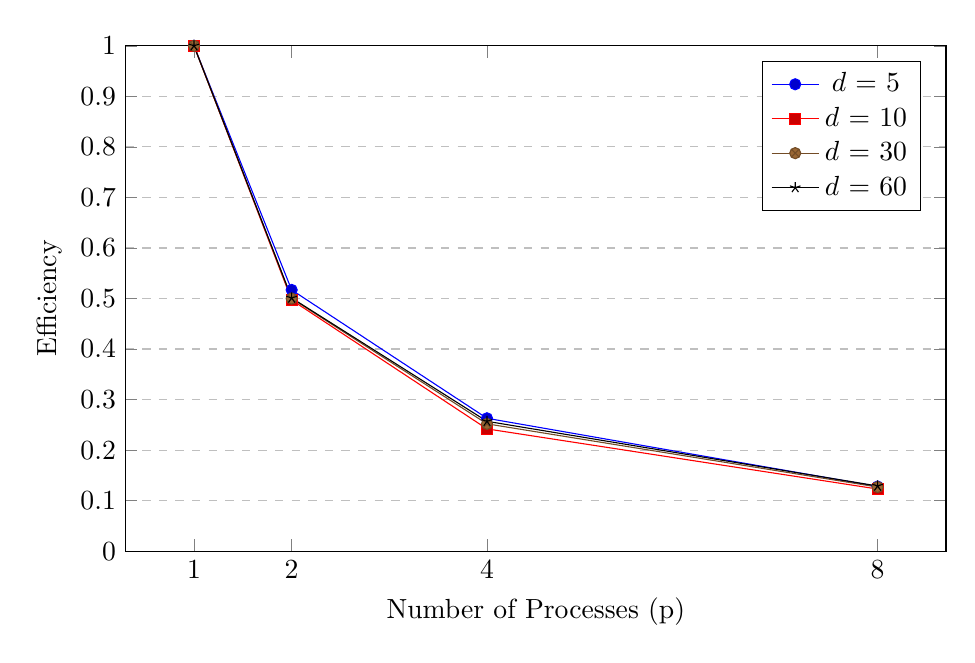
\begin{tikzpicture}
\begin{axis}[
    ylabel={Efficiency},
    xlabel={Number of Processes (p)},
    xticklabels={1,2,4,8},
    xtick={1,2,4,8},
    ytick={0.0, 0.1, 0.2, 0.3, 0.4, 0.5, 0.6, 0.7, 0.8, 0.9, 1.0},
    legend pos=north east,
    ymajorgrids=true,
    grid style=dashed,
    width=12cm,
    height=8cm,
    ymax=1,
    ymin=0,
]
\addplot coordinates {(1,1) (2,0.517) (4,0.263) (8,0.128)};
\addplot coordinates {(1,1) (2,0.497) (4,0.242) (8,0.123)};
\addplot coordinates {(1,1) (2,0.500) (4,0.252) (8,0.127)};
\addplot coordinates {(1,1) (2,0.501) (4,0.257) (8,0.129)};
\legend{$d$ = 5, $d$ = 10, $d$ = 30, $d$ = 60}
\end{axis}
\end{tikzpicture}
\caption{Efficiency for different problem sizes and process counts. $d$ is the loaded signal duration in minutes.}
\label{fig:judasefficiency}
\end{figure}

%\begin{figure}[!h]
%    \centering
%    \includegraphics[scale=0.5]{figures/speedup_judas.png}
%    \caption{Heatmap of speedups with Judas compared to serial execution}
%    \label{fig:ex2judheat}
%\end{figure}
\subsection{Experiment \rnum{2}: Parallel Resampling}

\begin{figure}[!htbp]
\centering
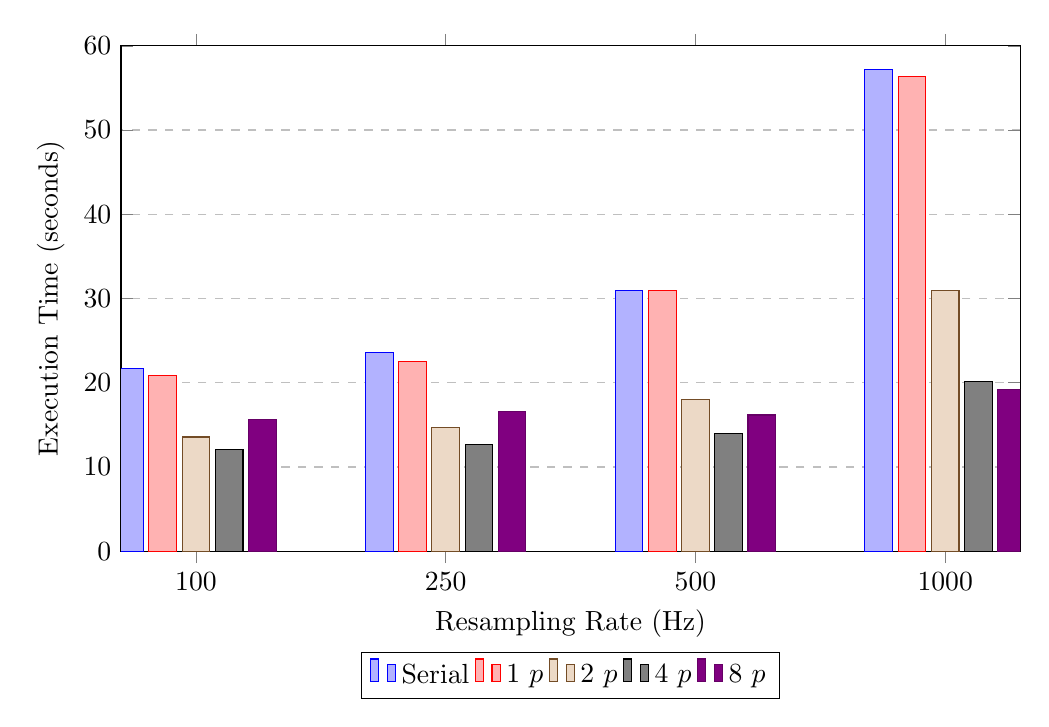
\begin{tikzpicture}
\begin{axis}[
    ylabel={Execution Time (seconds)},
    xlabel={Resampling Rate (Hz)},
    xticklabels={1000, 500, 250, 100},
    xtick={1000,500,250,100},
    legend pos=north west,
    ymajorgrids=true,
    grid style=dashed,
    width=13cm,
    height=8cm,
    bar width=10pt,
    ybar,
    legend style={at={(0.5,-0.20)},
    anchor=north,legend columns=-1},
    symbolic x coords={1000, 500, 250, 100},
    x dir=reverse,
    ymin=0, ymax=60,
]
\addplot coordinates {(1000,57.205) (500,30.970) (250,23.580) (100,21.695)};
\addplot coordinates {(1000,56.351) (500,30.941) (250,22.491) (100,20.843)};
\addplot coordinates {(1000,30.956) (500,17.998) (250,14.719) (100,13.556)};
\addplot coordinates {(1000,20.125) (500,13.937) (250,12.698) (100,12.066)};
\addplot coordinates {(1000,19.217) (500,16.173) (250,16.604) (100,15.619)};
\legend{Serial, 1 $p$, 2 $p$, 4 $p$, 8 $p$}
\end{axis}
\end{tikzpicture}
\caption{Execution times for different resampling rates and process counts ($p$). \footnote{Got help from Claude AI with spacing between bars}}
\label{fig:resampling-benchmark}
\end{figure}

\begin{figure}[!h]
    \centering
    \includegraphics[scale=0.5]{figures/speedup_heatmap(1).png}
    \caption{Speedups of the parallel resample function compared to serial execution. Green values mean higher speedups.}
    \label{fig:ex2heat}
\end{figure}

\begin{figure}[!htbp]
\centering
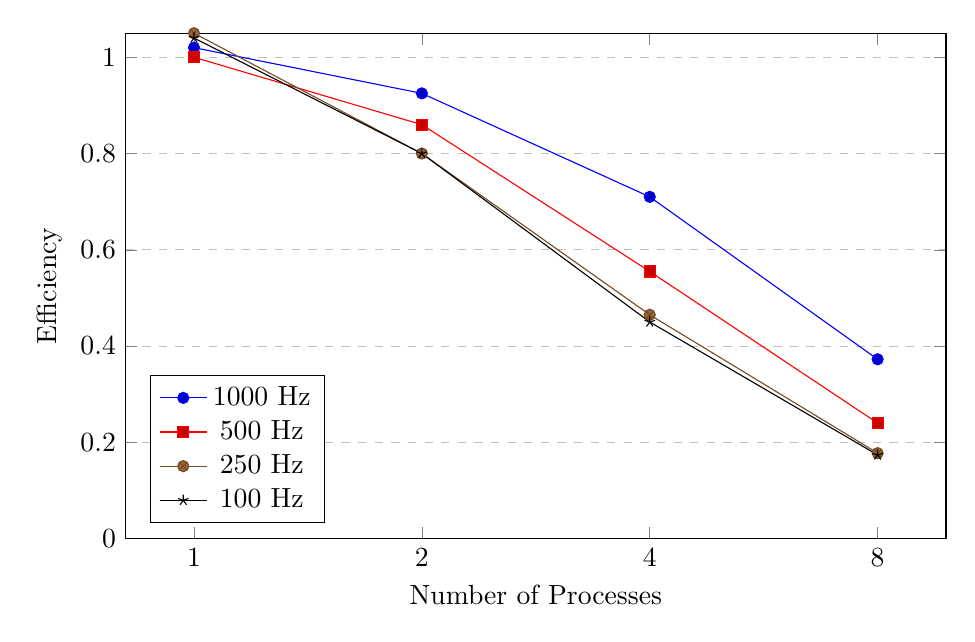
\begin{tikzpicture}
\begin{axis}[
    ylabel={Efficiency},
    xlabel={Number of Processes},
    xticklabels={1,2,4,8},
    xtick={1,2,3,4},
    legend pos=south west,
    ymajorgrids=true,
    grid style=dashed,
    width=12cm,
    height=8cm,
    ymax=1.05,
    ymin=0,
]
\addplot coordinates {(1,1.02) (2,0.925) (3,0.71) (4,0.3725)};
\addplot coordinates {(1,1.00) (2,0.86) (3,0.555) (4,0.24)};
\addplot coordinates {(1,1.05) (2,0.80) (3,0.465) (4,0.1775)};
\addplot coordinates {(1,1.04) (2,0.80) (3,0.45) (4,0.17375)};
\legend{1000 Hz, 500 Hz, 250 Hz, 100 Hz}
\end{axis}
\end{tikzpicture}
\caption{Efficiency Graph of the \texttt{das\_resample} function}
\label{fig:resampling_efficiency}
\end{figure}


\section{FORESEE}
\label{res:tinydas}

\subsection{Experiment \rnum{1}: Model training and Reconstruction}

\begin{table}[!htbp]
    \centering
    \small
    \setlength{\tabcolsep}{10pt}
    \begin{tabular}{l S[table-format=1.3e-2] S[table-format=2.1] S[table-format=1.3e-2] S[table-format=1.1e-3]}
        \toprule
        \rowcolor{gray!20}
        \textbf{Metric} & {\textbf{AE}} & {\textbf{$\beta$-VAE}} & {\textbf{CAE}} & {\textbf{$\beta$-CVAE}} \\
        \midrule
        Best Train loss & 1.300e-6 & 21.3 & 1.370e-4 & 4.5e-3 \\
        \rowcolor{gray!10} Best Validation loss & 1.300e-6 & 21.3 & 5.400e-5 & 4.4e-3 \\
        Epochs before stop & 6 & 20 & 15 & 15 \\
        \rowcolor{gray!10} Model Sizes & {\SI{10.240}{\giga\byte}} & {\SI{11.200}{\giga\byte}} & {\textbf{\SI{0.18}{\mega\byte}}} & {\textbf{\SI{47.06}{\mega\byte}}} \\
        Inference speed F32 (\si{\milli\second}) & 1.658 & 654.14 & 267.31 & 979.52 \\
        \rowcolor{gray!10} Inference speed F16 (\si{\milli\second}) & 1.875 & 6.31 & 5.671 & 1.857 \\
        \bottomrule
    \end{tabular}
    \caption{Comparison of Autoencoder Performance}
    \label{tab:modelresinfo}
    \smallskip
    \small{*The reconstruction error is the sum of all reconstruction errors across all batches.}
\end{table}


\begin{figure}[!h]
    \centering
    \includegraphics[scale=0.35]{figures/time.png}
    \caption{Comparison between Maximum and mediant amount of time spent per epoch}
    \label{fig:traintimes}
\end{figure}

\clearpage

\subsubsection{Train and Validation Losses}

\begin{figure}[!h]
  \centering
  \begin{subfigure}[t]{.6\textwidth}
    \centering
    \includegraphics[width=\linewidth]{figures/losses/ae.png}
    \caption{AE}
  \end{subfigure}
  \hfill
  \begin{subfigure}[t]{.6\textwidth}
    \centering
    \includegraphics[width=\linewidth]{figures/losses/ae.png}
    \caption{$\beta$-VAE}
  \end{subfigure}
  
  \vspace{1cm}
  
  \begin{subfigure}[t]{.6\textwidth}
    \centering
    \includegraphics[width=\linewidth]{figures/losses/ae.png}
    \caption{CAE}
  \end{subfigure}
  \hfill
  \begin{subfigure}[t]{.6\textwidth}
    \centering
    \includegraphics[width=\linewidth]{figures/losses/ae.png}
    \caption{$\beta$-CVAE}
  \end{subfigure}
  \label{fig:losses}
  \caption{Train and Validation Loss over Time}
\end{figure}

\clearpage

\subsubsection{Heatmap Reconstruction Comparison}

\begin{figure}[!h]
\centering
% Row 0 (Image Names)
\begin{subfigure}{0.33\textwidth}
\centering
2019-04-15 03:17:35
\end{subfigure}%
\hfill
\begin{subfigure}{0.33\textwidth}
\centering
2019-04-15 03:17:50
\end{subfigure}%
\hfill
\begin{subfigure}{0.33\textwidth}
\centering
2019-04-15 03:17:55
\end{subfigure}

    \vspace{1em}
    
    % Row 1 (Original)
    \begin{subfigure}{0.33\textwidth}
        \includegraphics[width=\textwidth]{figures/anomalies/before/20190415_031735.png}
    \end{subfigure}%
    \hfill
    \begin{subfigure}{0.33\textwidth}
        
\includegraphics[width=\textwidth]{figures/anomalies/before/20190415_031750.png}
    \end{subfigure}%
    \hfill
    \begin{subfigure}{0.33\textwidth}
        
\includegraphics[width=\textwidth]{figures/anomalies/before/20190415_031755.png}
    \end{subfigure}
    
    \vspace{1em}
    
    % Row 2 (Model 1)
    \begin{subfigure}{0.33\textwidth}
        \includegraphics[width=\textwidth]{figures/anomalies/ae/20190415_031735.png}
    \end{subfigure}%
    \hfill
    \begin{subfigure}{0.33\textwidth}
        
\includegraphics[width=\textwidth]{figures/anomalies/ae/20190415_031750.png}
    \end{subfigure}%
    \hfill
    \begin{subfigure}{0.33\textwidth}
        
\includegraphics[width=\textwidth]{figures/anomalies/ae/20190415_031755.png}
    \end{subfigure}
    
    \vspace{1em}
    
    
    % Row 4 (Model 3)
    \begin{subfigure}{0.33\textwidth}
        \includegraphics[width=\textwidth]{figures/test.png}
    \end{subfigure}%
    \hfill
    \begin{subfigure}{0.33\textwidth}
        \includegraphics[width=\textwidth]{figures/test.png}
    \end{subfigure}%
    \hfill
    \begin{subfigure}{0.33\textwidth}
        \includegraphics[width=\textwidth]{figures/test.png}
    \end{subfigure}


    \vspace{1em}
    
    % Row 3 (Model 2)
    \begin{subfigure}{0.33\textwidth}
        \includegraphics[width=\textwidth]{figures/anomalies/cae/20190415_031735.png}
    \end{subfigure}%
    \hfill
    \begin{subfigure}{0.33\textwidth}
        
\includegraphics[width=\textwidth]{figures/anomalies/cae/20190415_031750.png}
    \end{subfigure}%
    \hfill
    \begin{subfigure}{0.33\textwidth}
        
\includegraphics[width=\textwidth]{figures/anomalies/cae/20190415_031755.png}
    \end{subfigure}
    
    
    \vspace{1em}
    
    % Row 5 (Model 4)
    \begin{subfigure}{0.33\textwidth}
        \includegraphics[width=\textwidth]{figures/test.png}
    \end{subfigure}%
    \hfill
    \begin{subfigure}{0.33\textwidth}
        \includegraphics[width=\textwidth]{figures/test.png}
    \end{subfigure}%
    \hfill
    \begin{subfigure}{0.33\textwidth}
        \includegraphics[width=\textwidth]{figures/test.png}
    \end{subfigure}
    
    \caption{Comparison of original heatmaps and their reconstructions by different mdoels. The top row consist of original \acrshort{das} heatmaps, followed by reconstructions produced by: AE, $\beta$-VAE, CAE and $\beta$-CVAE}
    \label{fig:aereconstruct}
\end{figure}

\subsection{Experiment \rnum{2}: Anomaly Detection}

Table \ref{tab:confusion-matrix-results} presents a comparative analysis of all four models. The $\beta-CVAE$ has the highest values for the positives and the lowest of the negatives.

\begin{table}[!htbp]
\centering
\begin{tabular}{l
    S[table-format=3.0]
    S[table-format=3.0]
    S[table-format=3.0]
    S[table-format=3.0]
}
\toprule
\textbf{Model} & {\textbf{TP}} & {\textbf{FP}} & {\textbf{TN}} & {\textbf{FN}} \\
\midrule
\rowcolor{gray!10} AE   & 0 & 42 & 418 & 140 \\
$\beta$-VAE  & 101 & 2 & 458 & 39 \\
\rowcolor{gray!10} CAE  & 75 & 9 & 451 & 65 \\
$\beta$-CVAE & \textbf{103} & \textbf{5} & \textbf{455} & \textbf{37} \\
\bottomrule
\end{tabular}
\label{tab:confusion-matrix-results}
\caption{Confusion Matrix Values for all four models}
\end{table}


\begin{table}[!htbp]
\centering
\label{tab:performance-metrics}
\begin{tabular}{l
    S[table-format=1.3]
    S[table-format=1.3]
    S[table-format=1.3]
    S[table-format=1.3]
    S[table-format=1.3]
}
\toprule
\textbf{Model} & {\textbf{Precision}} & {\textbf{Recall (TPR)}} & {\textbf{F1-Score}} & {\textbf{FPR}} & {\textbf{PR AUC}} \\
\midrule
\rowcolor{gray!10} AE   & 0.000 & 0.000 & 0.000 & 0.091 & 0.157 \\
$\beta$-VAE  & \textbf{0.981} & 0.721 & \textbf{0.831} & \textbf{0.004} & \textbf{0.925} \\
\rowcolor{gray!10} CAE  & 0.893 & 0.536 & 0.670 & 0.020 & 0.736 \\
$\beta$-CVAE & 0.954 & \textbf{0.736} & \textbf{0.831} & 0.011 & 0.924 \\
\bottomrule
\end{tabular}
\label{tab:auto}
\caption{Anomaly Detection Performance Metrics Comparison}
\end{table}



\begin{figure}[!htbp]
    \centering
    \begin{subfigure}[b]{\textwidth}
        \centering
        \includegraphics[width=0.8\textwidth]{figures/anomalies/combined_roc_curve.png}
        \caption{Combined ROC Curve for all models}
        \label{fig:roccurve}
    \end{subfigure}
    \vspace{1em}
    \begin{subfigure}[b]{\textwidth}
        \centering
        \includegraphics[width=0.8\textwidth]{figures/anomalies/combined_pr_curve.png}
        \caption{Combined PR Curve for all models}
        \label{fig:prcurve}
    \end{subfigure}
    \caption{Performance curves for all models}
    \label{fig:combined_curves}
\end{figure}
\clearpage

\subsubsection{Threshold Analysis}

\begin{figure}[!h]
  \centering
  \includegraphics[scale=0.5]{figures/anomalies/ae/threshold.png}
  \caption{Threshhold analysis for the AE model}
  \label{fig:threshold_ae}
\end{figure}

\begin{figure}[!h]
  \centering
  \includegraphics[scale=0.5]{figures/anomalies/vae/threshold.png}
  \caption{Threshhold analysis for the $\beta$-VAE model}
  \label{fig:threshold_vae}
\end{figure}

\begin{figure}[!h]
  \centering
  \includegraphics[scale=0.5]{figures/anomalies/cae/threshold.png}
  \caption{Threshhold analysis for the CAE model}
  \label{fig:threshold_cae}
\end{figure}

\begin{figure}[!h]
  \centering
  \includegraphics[scale=0.5]{figures/anomalies/cvae/threshold.png}
  \caption{Threshhold analysis for the $\beta$-CVAE model}
  \label{fig:threshold_vae}
\end{figure}


Clearbout \cite{claerbout1991scrutiny}
Landes scrutiny \cite{landes1951scrutiny}
omar2013 machine \cite{omar2013machine}
wei lstm autoenc \cite{wei2022lstmautoencoder}
apsensing railways \cite{apSensing2019railwaydas}
srivatavams15 \cite{DBLP:journals/corr/SrivastavaMS15}
2011 ndonssigprocandet \cite{2011ndongsigprocandet}
doi101136141000671 \cite{doi:10.1137/141000671}
bioeng \cite{bioengineering10040405}
maulik2020recurr \cite{maulik2020recurrent}





\chapter{Discussion}
\label{chap:disc}

This sixth chapter analyzes the results presented in Chapter \ref{chap:results} and further examines the programs detailed in Chapter \ref{chap:exp}. We explore the overall design, strengths, and current limitations of both \texttt{Judas} and \texttt{TinyDAS}. The chapter concludes with an evaluation of Julia as a programming language for data science and \acrshort{ai} applications.


\section{Discussion}
\label{chap:discussion}

\section{Modularity in Data Science}

api design for data science has for far long enough been overlooked. Full AI models are regularly being comprised in a single file, with only a argument parser to make sure python can run the script. We instead wanted to seperate between the different aspects of the AI part of the code. The models, engine and hyperparameters can all easily be split into multiple files, but yet this is not common. The advantage we gain by splitting up this module, is easier ways of debugging, as well as to more easily reuse only the sections of the code that we're interested in. Training and Inference are by default split in their own files, since we don't actually want those two run after each other. The training of the neural net should only happen when needed, inference is the mode we'd actually like to test against and return the answers about loss and so on 


\section{Interpretibility}
One major question we wanted to tackle is regarding interpretibility. Is this achieved, or do we still have a long way to go?
\section{Reflections on Julia}
\label{sec:juliaref}

Intro

Since the very first day of this project, we've been using Julia quite rigorously. Some may argue that C and Python would be more efficient due to their extensive ecosystems and documentations. They are also more or less the \textit{de-facto standard} programming languages for their respective fields, \acrshort{hpc} and \acrshort{ai}. Additionally, members of \acrshort{cgf} are more accustomed to these languages, so why Julia? \\

Besides what's already been mentioned, we wanted to give our thoughts on developing in Julia. Before getting started with Julia as the target language of our program, we made sure it had all the different packages we would need. For \acrshort{ai} and \acrshort{ml} packages, we were pleasantly surprised to find multiple options that all perform well. Bindings to similar packages in Python could also easily be found. We opted for Flux, and with its native integration with CUDA, no extra work had to be done to make use of \acrshort{gpu}s to speed up the computation of our models.

One of the best \\ 
Next to this comes the builtin \texttt{@inbounds} macro, which turns of the boundary checker when accessing memory, speeding up computations in a short matter of time. Not only this, but all the different macros in Julia were pleasant to work with. \texttt{time}, \texttt{btime}, \texttt{profile}, \texttt{cuda}, \texttt{btime}, \texttt{simd} all help imensly when creating programs, without the need for writing loops or custom instructions. Just simply knowing how and where to place macros cleans up the code, and not only increases the developer experience, but also standardizes code between codebases without having to rewrite all from scratch. Just simply running and launcing cudakernels as in \ref{app:jlvsc} shows how easy it is to setup and run CUDA kernels as long as the \texttt{CUDA.jl} package is installed. \\

Version control
A majority of new languages and compilers comes with a version multiplexer, examples being \texttt{rustup}, \texttt{}. These are not built retrospectively, as is the case for \texttt{sdkman} for Java, but before. Managing dependencies and packages, maintaining larger programs and so on becomes a lot easier with both a version multiplexer and a productive package manager. C has never had a standard way of dealing with packages, and this has inspired future languages to extend their ecosystems to include this alongside the compiler and standard library. Python has \texttt{PyPI}, but with many different programs to deal with versioning and packages. Some of these are venv, \texttt{Anaconda} and \texttt{Poetry}. Just simply installing and setting up projects in these languages seem to be harder than it actually have to be, and Julia proves this. \\ 

Enabling multiple processors or threads comes down to simply specifying a flag when running \texttt{-p} or \texttt{-t} respectively. The language has these kinds of computing built into the standard library, no need to install third party dependencies. 

When it comes to AI, Python has stayed supreme as the \textit{de-facto standard} for implementing and testing models. Tensorflow, Pytorch and recently Tinygrad are all highly optimized frameworks for working with ML, with thousands of articles, papers and learning materials written about them. Comparatively, Julias \texttt{Flux.jl} is way younger, but offers in our opinion, easier GPU toggling, model design and overall a smoother experience for . The docs of Flux.jl takes one through the entire codebase, and after reviewing models on \cite{https://github.com/FluxML/model-zoo}, it's easy to figure out how to setup, train and save models.

Julia excels when it comes to scientific computations. Not only does the suppport of unicode symbols make it easier to translate whitepapers to code, but Julias syntax and its compilation makes for an incredible developer experience, as well as increased performance. In the appendix, one can see an example of plotting in Julia, and how intuitive it can be, compared to other languages.






Cons
Although Julia has shown to have many strengths, there is no thing such as a perfect programming language. Julias' main weaknesses besides a far younger ecosystem compared to its alternatives, is its lack of documentation. 

Another potential drawback is the relatively young ecosystem for \acrshort{ai} or \acrshort{ml} programmming that exits compared to Python. As mentioned in \ref{chap:back}, Julia has bindings for Tensorflow, yet still Flux is preferred in most cases. Although it seems to have all functions necessary for computations, some of its functions are not as optimized as they can be. As discussed in \cite{projthesis}, \lstinline|relu| was not optimized until the end of last year. These kinds of optimizations, be it trivial or not, will impact larger programs on a significat level, so we might want to benchmark certain functions to see if they may be optimized futher. However, this is also a great aspect of Julia. Since Flux is natively written in Julia, replacing old functions with more optimized or type specific functions seem to  


Conclusions on personal use 
\chapter{Conclusion and Further work}
\label{chap:conclusion}

This final chapter summarizes the key findings of our research. We present our conclusions, evaluate the extent to which we've reached our goals, and discuss the broader implications of our work. The chapter concludes by exploring potentials for further work, building upon the foundation laid by this thesis.

\section{Conclusion}
\label{conc:conc}

\acrshort{das} processing is a complex task requiring many precise calculations. The massive amounts of stored data have also highlighted the need for more efficient file loading, processing, and analysis algorithms. In this thesis, we provide tools for improved efficiency in processing and analyzing \acrshort{das} data and a comparative analysis of different autoencoder architectures. By developing
Judas and TinyDAS, we bridge the gap between pre-processing \acrshort{das} data and anomaly detection by providing a direct pipeline between the two as shown in Figure \ref{fig:judasnet_overview}. Furthermore, these tools can be used for future research by members at \acrshort{cgf} and other researchers.

For Judas, we argue the case for looking at recent advancements in programming language design and parallel techniques further to enhance efficiency in \acrshort{das} processing. Although our current file loading is still slow, the reduced memory requirements, temporary file storage, and on-demand loading allow for more efficient handling of large-scale dense-sampled \acrshort{das} data.

As for TinyDAS, we reached our goals in terms of providing software for comparative analysis of autoencoder-based anomaly detection and hardware-agnostic model training, as discussed in Section \ref{disc:tinydas}. Our comparisons demonstrate the usefulness of smaller convolutional architectures as viable options, even in large-scale spatial data.

Even though the topic of this thesis has been broad and contains several aspects, we were able to condense our research into three main questions. Following are the answers to these research questions:

\textbf{RQ1: How do the spatial characteristics of large-scale dense-sampled \acrshort{das} data impact the anomaly detection performance using autoencoders?}
The distinct difference in especially reconstruction capabilities, as well as anomaly metrics (e.g., F1 score, specificity, and precision) between the linear and convolutional models, further indicates the importance of capturing spatial characteristics within \acrshort{das} data for enhanced performance in anomaly detection. Our results show that simple convolutional autoencoders outperform the dense autoencoders, highlighting the critical role of extracting spatial characteristics in \acrshort{das} anomaly detection.

\textbf{RQ2: How does half-precision inference affect anomaly detection in \acrshort{das} data?}:
 We effectively reduce inference time cost by a mean factor of \textit{170} across our models by using half-precision inference. Furthermore, our research does not indicate any significant shortcomings by utilizing half-precision for anomaly detection in \acrshort{das} data, but this may vary case-by-case. These points present a vital point about testing out half-precision, especially for real-time environments.

\textbf{RQ3: How can we make the entire data processing pipeline, from loading \acrshort{das} data to detecting anomalies, as fast and efficient as possible?} The pipeline from finding and loading \acrshort{das} data to detecting anomalies may seem long and tedious. Still, our research discusses and provides several different techniques for efficient handling of \acrshort{das} data, including:

\begin{enumerate}
    \item Memory Management and Parallel Processing
    \begin{itemize}
        \item Utilize parallel file loading
        \item Divide \acrshort{das} data into smaller matrices for distributed processing
        \item Leverage temporary file storage
        \item Implement parallel channel decimation
    \end{itemize}
    \item Model Optimization and Training
    \begin{itemize}
        \item Design models with the spatial characteristics in mind
        \item Test out simpler architectures before larger and more complex architectures
        \item Store weights and biases in single-precision to capture the minute details of \acrshort{das} data
    \end{itemize}
    \item Anomaly detection
    \begin{itemize}
        \item Utilize half-precision for faster prediction
        \item Allow for some non-anomalous data to make the model more robust to noise and minimize manual intervention
        \item Focus on detecting anomalies in smaller windows
        \item Compare and test several models on a case-by-case scenario
    \end{itemize}
\end{enumerate}

In conclusion, our research has contributed to the field of \acrshort{das} data analysis by developing efficient tools and identifying effective strategies for anomaly detection. We've demonstrated the importance of considering spatial characteristics, compact convolutional architectures' potential, and the benefits of strategic preprocessing techniques. Even though not all methods proved positive, this work has proven both meaningful and productive. As the field continues to evolve, the tools and insights provided by this thesis offer a solid foundation for ongoing advancements in \acrshort{das} data processing and analysis.


%\textbf{RQ2: What autoencoder architectures are most effective for anomaly detection in \acrshort{das} data when computational resources can be limited?}
%
%Although the convolutional models require a smaller batch size as of now, thus leading to higher training, based on median epoch duration and the epoch count seen in Table \ref{tab:modelresinfo}, combined with the significantly smaller model sizes, improved anomaly scores, and overall reconstruction capabilities, we find simpler convolutional models, such as our CAE model, to be sufficiently effective. These models balance computational efficiency and detection performance, making them well-suited for scenarios where computational resources are scarce.
%
\section{Further work}
\label{conc:further}

While our work has addressed several key challenges, both Judas and TinyDAS are in their first iterations. Further research and development can address the current limitations discussed in this thesis.

\subsection{Judas and \acrshort{das} processing}

While Judas serves the task of loading and processing \acrshort{das} data, the following list provides an overview of further advancements that can enhance its computational effectiveness, specifically targeting file loading:

\begin{itemize}
    \item Design and implement a more course-grained approach to our current solutions for finding and loading \acrshort{das} files. 
    \item Designing a parallel version of the column-wise cumulative sum function, potentially using algorithms like parallel prefix sum \cite{harris2007parallel}, where \acrshort{gpu} acceleration could be introduced. 
    \item Implementing a more flexible metadata handling system to accommodate datasets from other sources besides BANENOR.
    \item Implementing more advanced denoising and signal processing techniques, potentially utilizing denoising autoencoders \cite{eage:/content/journals/10.1111/1365-2478.13355}.
\end{itemize}

\subsection{TinyDAS and Autoencoder-based Anomaly Detection}

As discussed in Section \ref{disc:tinydas}, we have succeeded in many of our goals with TinyDAS. However, as the poor results from the variational autoencoders show, there is still much room left for tuning current models. The following list presents multiple avenues for further development and research:

\begin{itemize}
    \item Expand support for more different architecture and compare simpler models with hybrid models that combine both the temporal and spatial aspects of \acrshort{das} signals, such as CNN-LSTM architectures, or even transformer-based ones, to capture finer details.
    \item  Half-precision training has been a heavy area of attention. For now, TinyDAS supports half-precision training, inference, loss-scaling, and gradient clipping. Further improving on these to ensure gradients are within range is an important aspect of reducing runtime and memory consumption. Comparing this approach to mixed-precision could prove beneficial.
    \item Expanding support for other \acrshort{das} datasets, both from PubDAS and other public sources. This could be achieved through a more customizable format of our DataLoader class. Furthermore, implementing functionality for downloading \acrshort{das} datasets directly from the internet would lower the user entry barrier.
    \item Implement support for reading real-time datastreams, to further analyze how different models perform in real-world scenarios
\end{itemize}

\subsection{Final Remarks}

We want to thank \acrfull{cgf} for providing data and computational resources. We hope both these programs can help all their current and future members further the field of \acrshort{das} research.



\chapter*{\bibname}
\printbibliography[heading=none]

\appendix
\chapter{Julia}
\label{app:julia}

\section{CUDA in Julia vs C}
\label{app:jlscicomp}

\begin{figure}[!h]
    \centering
    \lstinputlisting[language=Julia]{code/jlcuda.jl}
    \caption{Launching CUDA kernel in Julia. This can be run directly with the Julia compiler}
    \label{fig:jlcuda}
\end{figure}
 
\lstinputlisting[language=C, label={fig:ccuda}]{code/ccuda.c}

\section{MNIST in Julia}

\lstinputlisting[language=Julia, caption=MNIST in Julia, label={code:juliamnist}]{code/mnist.jl}

\section{Autoencoder Julia Example}

\lstinputlisting[language=Julia, caption=Dense Autoencoder with one hidden layer implemented in Julia using the \texttt{Flux.jl} package, label={code:judasnet}]{code/judasnet.jl}
\chapter{Judas}
\label{app:judas}


\section{Packages Used}
\label{app:jupacks}

\begin{table}[!h]
\centering
\caption{Packages used in Judas}
\label{tab:judas-packages}
\small
\begin{tabular}{>{\raggedright\arraybackslash}p{0.25\textwidth}>{\raggedright\arraybackslash}p{0.65\textwidth}}
\toprule
\textbf{Package Name} & \textbf{Description} \\
\midrule
%\rowcolor{gray!10} Flux & AI library \\
CUDA & NVIDIA CUDA programming \\
\rowcolor{gray!10} DSP & Digital Signal Processing \\
DataFrames & Working with Dataframes \\
\rowcolor{gray!10} JLD2 & Saving and loading of models \\
HDF5 & HDF5 wrapper for Julia \\
\rowcolor{gray!10} LinearAlgebra & Linear Algebra package \\
Statistics & Distributions and common functions for statistics\\
\rowcolor{gray!10} Mmap & Memory mapped I/O for working with large arrays \\
Distributed & Parallel computing in Julia \\
\rowcolor{gray!10} FFTW & FFTW wrapper for Julia \\
Dates & Datetime library \\
\rowcolor{gray!10} Plots & Plotting utilities \\
Colors & Extra colorschemes for plots \\
\rowcolor{gray!10} BenchmarkTools & Benchmark tools and utilities \\
SymPy & Julia wrapper for working with symbolic notation \\
\bottomrule
\end{tabular}
\end{table}

\section{Load DAS Files function}
\label{app:loaddas}
\lstinputlisting[label={code:loaddas},caption=Load DAS Files, language=Julia]{code/loaddas.jl}
\chapter{PubDAS Foresee Data Preprocessing}
\label{app:pubdas}

\lstset{style=pstyle}
\lstinputlisting[language=Python, caption=Preprocessing of the FORESEE dataset from TDMS to HDF5]{code/pubdas.py}
\chapter{TinyDAS: Experiment Setup}
\label{app:tinydas-exp}

\lstinputlisting[language=Python, caption=Experiment setup for measuring Autoencoders, label={app:adreport}]{code/ad.py}

\chapter{Trainmap BaneNOR}
\label{app:jlscicomp}

\begin{figure}[h]
    \centering
    \includegraphics[scale=0.5]{figures/togkart.png}
    \caption{Map over train route from Trondheim to Storen}
    \label{fig:trainmap}
\end{figure}

\end{document}
